\chapter{Statistics tool box}
\label{chap:stat}

The result of a \gls{pp} interaction is not deterministic, as the statements that can be obtain from quantum field theory are of probabilistic nature. 
Furthermore, uncertainties in our predictions related both to experimental effects and to the modelling of the physics processes need to be taken into account. 
Therefore, a proper statistical treatment is essential to extract quantitative statements from the observed data. 
%This chapter does not aim at being an exhaustive reference for statistics, but it 
This chapter describes the main statistical procedures that are used to obtain the results described in Chapter \ref{chap:strong_prod} and Chapter \ref{chap:ewk_prod}. After a brief introduction to statistical inference in Section \ref{sec:stat:intro}, the two main topics discussed are parameter estimation, in Section \ref{sec:stat:pe}, that has the aim to determine the value of the input parameters that allows to best describe data, and hypothesis testing, in Section \ref{sec:stat:ht}, that checks the plausibility of models against the observed data. 
Section \ref{sec:stat:examples} describes two simplified examples of applications of these statistical methods to physics analyses. 

%%%%%%%%%%%%%%%%%%%%%%%%%%%%%%%%%%%%%%%
\section{Statistical inference}
\label{sec:stat:intro}

Statistical inference uses a data sample to make probabilistic statements on the population from which the sample is extracted. The generalization from the properties of the sample to the properties of the entire population comes with a certain degree of uncertainty, that can also be accesses through statistical methods.
There are two main approaches to statistical inference: Bayesian and frequentist.

\begin{description}
\item[Frequentist] In the frequentist approach, probability is defined as the fraction of favorable outcomes of a repeatable experiment when the number of repetitions tends to infinity:
\begin{equation}
P(\mathrm{A}) = \lim_{N_{\mathrm{tot}} \rightarrow \infty} \frac{N_\mathrm{A}}{N_{\mathrm{tot}}} \; .
\end{equation}
In this case there is no probability for hypothesis or true values of the parameters: a theory is either true or false, and given a theory only the data has a certain probability or \gls{pdf}.

\item[Bayesian] In the Bayesian approach, probability is a more subjective notion, that incorporates the degree of belief in the from of priors. In this case it is meaningful to speak about \gls{pdf} not only for the observed data, but also for theories and parameters. Performing an experiment will modify the probability of a theory according to the Bayes formula:
\begin{equation}
P(\mathrm{theory} | \mathrm{data}) = \frac{ P(\mathrm{data}|\mathrm{theory}) \times P(\mathrm{theory})}{P(\mathrm{data})} \; ,
\end{equation}
where $P(\mathrm{data}|\mathrm{theory})$ is the probability of the data given the theory under examination, $P(\mathrm{theory})$ is the theory prior, $P(\mathrm{data})$ is a normalization constant that expresses the probability of observing these data whether the theory is true or false, and $P(\mathrm{theory} | \mathrm{data})$ is the final posterior probability of the theory.

\end{description}

In this chapter we discuss only about frequentist statistics, as only frequentist methods are applied to obtain the results presented in chapters \ref{chap:strong_prod} and chapter \ref{chap:ewk_prod}. 

As mentioned above, an hypothesis is a statement based on which one can access the probability of the data. An hypothesis can be simple, when the data \gls{pdf} can be fully determined by stating if the hypothesis is true or false, or complex, when it depends on a number of parameters that in the following will be generally denoted with $\theta$. 

Given a certain hypothesis $H$, the probability of observing the data $x$ is $P(x|H)$. This probability can be considered also as a function of the hypothesis, for fixed data, and in this case it is assigned the name of likelihood ($L$). In the case of a composite hypothesis, the value of the likelihood depends on the value of the parameters necessary to specify the hypothesis, and it takes the name of likelihood function: $L(\theta)=P(x|\theta)$.

\section{Parameter estimation}
\label{sec:stat:pe}

Parameter estimation, also know as fitting, is the technique that allows to derive the best values of some parameters from data.
This sections describes parameter estimation and in particular the method based on the maximum likelihood.

\subsection{Estimators}

Consider a set of independent observations $\vec{x}=\{x_1, x_2, ..., x_\mathrm{N}\}$, distributed accordingly to a \gls{pdf} $f(x|\vec{\theta})$, where $\vec{\theta}=\{\theta_1, \theta_2, ..., \theta_\mathrm{M}\}$ are the M true parameters that specify the underlying theory. 
A statistic is any function of the measured data $\vec{x}$, and an estimator $\hat{\vec{\theta}}$ is a statistic introduced to provide an estimate of $\vec{\theta}$.
The characteristics used to evaluate the performance of an estimator are:

\begin{description}
\item[Consistency] The asymptotic limit for large number of observations of the estimator is the true value of the parameter:
\begin{equation}
\label{eq:stat:consistency}
\lim_{N \rightarrow \infty} \hat{\vec{\theta}} = \vec{\theta} \; .
\end{equation}

\item[Bias] The bias is the difference between the expectation value of the estimator ($E[\hat{\vec{\theta}}]$) and the true value:
\begin{equation}
\label{eq:stat:bias}
b = E[\hat{\vec{\theta}}] - \theta \; .
\end{equation}
Once the bias of a specific estimator is known, it is possible to build and unbiased one by defining 
\begin{equation}
\hat{\vec{\theta}}_{\mathrm{unbiased}} = \hat{\vec{\theta}} - b \; .
\end{equation}

\item[Efficiency] The efficiency of an estimator is high when its variance ($V[\hat{\vec{\theta}}]$) is small. $V[\hat{\vec{\theta}}]$ has a lower bound, that is given by the Cramer-Rao inequality \cite{Cramer1946}\cite{Rao1992}.

%, stating that the variance is larger than the inverse of the information matrix $I[\theta]$
%\begin{equation}
%V[\hat{\vec{\theta}}] \geq I[\vec{\theta}]^{-1}
%\end{equation}

\item[Robustness] An estimator is robust if it is not sensitive to small changes in the assumptions in the \gls{pdf}.
\end{description}



\subsection{The maximum Likelihood estimator}
\label{sec:stat:MLE}

The \gls{mle} of the parameters $\theta_i$, first introduced by Fisher \cite{fisher1911absolute,aldrich1997}, is obtained by choosing the set of parameters that yields the global maximum of the likelihood function. At an intuitive level this corresponds to the choice for which the observed data $\vec{x}$ are more probable. 

The \gls{mle} is widely used because of the favorable properties that it reaches in the asymptotic limit of infinite number of events N:
\begin{itemize}
\item Consistent, which means that it satisfies Eq. \ref{eq:stat:consistency}.
\item Unbiased, so the bias, defined in Eq. \ref{eq:stat:bias}, tends to zero.
\item Efficient, as it reaches the minimum bound for the variance.
\item It follows a Gaussian distribution.
\end{itemize}

\noindent With a finite number of events, the estimator is biased and the bias is proportional to $\frac{1}{N}$. Also, the \gls{mle} is invariant under a functional transformation, which means that if $\hat{\theta}$ is the \gls{mle} for the parameter $\theta$, $g(\hat{\theta})$ is the \gls{mle} for the reparametrization $g(\theta)$, and it maintains therefore all the properties described above. This is not necessarily true for other estimators.

Practically, most of the times instead of maximizing the likelihood function is more convenient to minimize $-\logl$. This has the advantage to move from a maximization to a minimization because of the minus sign, but also to transform all the products into sums, which makes the minimization easier. As long as the likelihood is a monotonous function, its maxima are the same as the ones of the $\logl$.
There are two types of maximum likelihood fits that can be performed:

\begin{description}
\item[Unbinned fits] Each event enters in the likelihood separately. This method is the optimal one from the statistics point of view, but it results to be computationally expensive.
\item[Binned fits] The events are grouped in bins of a histogram, and the quantity entering in the likelihood is the number of events in each bin.
\end{description}

\noindent In this chapter the focus will be on the second type of fit, as it is the one used in this thesis.

\subsubsection*{Variance of the maximum Likelihood estimator}

The estimate of a parameter based on a data sample is always associated with an uncertainty.
The the same parameter estimate is performed on a different data sample, the values of the best estimate are different;
if this is repeated N times on independent data samples, for large N the best estimates will have a distribution that tends to a Gaussian, 
whose variance gives access to the uncertainty on the \gls{mle}. The two ways to access this variance are:

\begin{description}
\item[Monte Carlo method] Once the parameter is estimated from the experimental results, the experiment can be simulated N times with \gls{mc}  simulations. For each simulation the best value of the parameter can be estimated with the maximum likelihood method, and from the distribution of these values it is possible to compute the variance.

\item[Graphical method] With the increase of the size of the data sample, the likelihood function tends to a Gaussian, and the $\logl$ tends to a parabola, so the variance of the distribution can be obtained as the point where $-\logl = \frac{1}{2}$.

\end{description}


\subsection{Binned Likelihood with systematic uncertainties}

If we consider the representation of the observed data given by the binned distribution of a certain variable, the expected number of events in each bin of the distribution is given by:

\begin{equation}
\label{eq:stat:exp}
E[n_i] = b_i + \mu s_i  \; ,
\end{equation}

\noindent where $b_i$ is the expected number of background events, $s_i$ the expected number of signal events and $\mu$ the signal strength.
If the observed data follow a Poisson distribution, the likelihood is given by:

\begin{equation}
\label{eq:stat:lik_no_sys}
L(\mu) =
\prod_{i=1}^N \frac{ (\mu s_{i} +
b_{i} )^{n_{i}} }{ n_{i}! }
e^{- (\mu s_{i} + b_{i}) } \; ,
\end{equation}

\noindent where the index $i$ runs on all the bins of the distribution.

The prediction on the expected number of events in each bin is affected by systematic and statistical uncertainties, that are incorporated in the Likelihood in the form of \glspl{np}. 
In the frequentistic approach, each \gls{np} has a true unknown value, whose \gls{mle} derived in auxiliary measurements. 
While in principle the full likelihood of the auxiliary measurements should be included in the likelihood of our own measurement, 
in most practical cases this is not feasible, and the auxiliary likelihood is modelled through constraining terms. 
Assuming that data used to derive the constraints on the \glspl{np} is statistically independent from the data in the analysis and not affected by the potential presence of the signal under study, the combined likelihood assumes the factorized form:

\begin{equation}
\label{eq:stat:lik_sys}
L(\mu, \vec{\theta}) =
\prod_{i=1}^N \frac{ (\mu s_{i} +
b_{i}(\vec{\theta}) )^{n_{i}} }{ n_{i}! }
e^{- (\mu s_{i} + b_{i}(\vec{\theta})) }   \;
\prod_{k=1}^M \rho( \theta_k) \; ,
\end{equation}

\noindent where $\rho( \theta_k)$ is the constraint term for the parameter $\theta_k$. Note that the treatment of an uncertainty through the addition of a constraint term, from the pure frequentist point of view is justified only for sources of uncertainty of experimental nature, where there is indeed an auxiliary measurement. The same approach is instead often used also for theoretical uncertainties, where the frequentist prescription would be to have a result that depends on these parameters. While in the Bayesian view the constrain term would easily be interpreted as a prior on the value of the theoretical parameter, in the frequentist approach this is equivalent to assigning also to the theoretical uncertainties a fictitious auxiliary measurement. 


\subsubsection*{Functional forms of the constraining terms}

Depending on the underlying auxiliary measurement, different functional types can be used for the constraining terms.

\begin{description}
\item[Gaussian constraint] This is the default constrain type for systematic uncertainties, and its usage is justified by the central limit theorem. In general, it is safe to use this constraint as long as the \gls{mle} of the \gls{np} from the corresponding auxiliary measurement follows a Gaussian distribution. The functional form is:

\begin{equation}
\label{eq:stat:gauss}
\rho( \theta) = \frac{1}{\sqrt{2\pi}\sigma}\exp\left( -\frac{(\theta - \hat{\theta})^2}{2\sigma^2} \right) \; .
\end{equation}

\noindent Technically, the function implemented in the likelihood is a truncated Gaussian, in order to avoid non-zero probability for non-physical values of the \gls{np}. This truncated Gaussian is normalized to still have unit area.

\item[Poisson constraint] This constraint is often referred to as "Gamma" constraint because, when using it in a Bayesian approach, if combined with a uniform prior it gives rise to a Gamma posterior. It is used for \glspl{np} related to event count and to model the \gls{mc} statistical uncertainty. If we assume that the background yield predicted from \gls{mc} is $n$ background events, deriving from $N$ \gls{mc} simulated events with a multiplicative scale $\alpha$, then the constraint term is:

\begin{equation}
\label{eq:stat:poisson}
\rho(n) = \frac{1}{\alpha} \frac{(n/\alpha)^N}{N!} \exp\left( -n/\alpha \right) \; .
\end{equation}

\item[Log-normal constraint] Log-normal is the distribution of a variable whose logarithm is distributed according to a Gaussian distribution. When random variables are multiplied, their product follows a log-normal distribution:

\begin{equation}
\label{eq:stat:lognorm}
\rho( \theta) = \frac{1}{\sqrt{2\pi}\ln{\sigma}}\exp\left( -\frac{(ln{\frac{\theta}{\hat{\theta}}})^2}{2(\ln{\sigma})^2} \right)\frac{1}{\theta} \; .
\end{equation}

\noindent One of the advantages of this constraint is that it never assumes negative values.

\end{description}



\subsubsection*{Evaluation of the response}

Let’s consider one single bin of a distribution and the effect that a systematic uncertainty has on it, e.g. the \gls{jer} uncertainty. 
Leaving aside the physical meaning of this uncertainty, we can focus on the effect that this calibration uncertainty has on the likelihood of a single bin counting experiment. 
The \gls{jer} uncertainty is calibrated with an auxiliary measurement, whose likelihood we include by the simplification of a Gaussian constraint term, $G( \tilde{\theta} | \theta, \sigma_\theta)$, where $\tilde{\theta}$ is the nominal value of the calibration, $\theta$ the underlying real value and $\sigma_\theta$ the uncertainty. Stating that the uncertainty on \gls{jer} is 10\%, means that the width of the Gaussian is 10\%. 

To include this information in the likelihood, we need to evaluate the response to this uncertainty, i.e. the effect of a shift in \gls{jer} in the background efficiency of our region.
In practice this means that we need to evaluate how much a one-sigma variation of \gls{jer} (10\% in our example) changes the number of expected events in the bin we are considering. 
For this example, we assume that a 10\% shift in \gls{jer} causes a 20\% change in the background yields.
If we consider only one bin of the likelihood in Eq. \ref{eq:stat:lik_no_sys}, consider only one systematic (\gls{jer} in this case) and write explicitly the effect of the systematic on the number of background events, we have:

\begin{equation}
\label{eq:stat:lik_one_bin_sys_pre}
L(\mu, \theta) =
\frac{ (\mu s +
b \left( \frac{\theta}{\tilde{\theta}} \right) 2 )^{n} }{ n! }
e^{- (\mu  + b\left(\frac{\theta}{\tilde{\theta} }\right)2)}   \; 
G( \tilde{\theta} | \theta, \sigma_\theta) \; .
\end{equation}

\noindent The change $b \rightarrow b\frac{\theta}{\tilde{\theta} }2$ encodes exactly the fact that a 10\% change in \gls{jer} leads to a 20\% change in background yields. To simplify this expression, the auxiliary measurement can be normalized to a standard Gaussian: $G( \tilde{\theta} | \theta, \sigma_\theta) \rightarrow G( 0 | \theta, 1)$, where also $\theta$ has been normalized such that the values $\theta = \pm 1$ correspond to the nominal uncertainty. The likelihood then becomes:


\begin{equation}
\label{eq:stat:lik_one_bin_sys}
L(\mu, \theta) =
\frac{ (\mu s +
b(1 + 0.1\theta) )^{n} }{ n! }
e^{- (\mu  + b (1 + 0.1\theta) )}   \;
G( 0 | \theta, 1) \; .
\end{equation}

\subsection*{Interpolation}

The response of the efficiency to a $\pm 1 \sigma$ variation of each parameter in the likelihood is something that is measured in each specific analysis. This process is done for only for three points (the nominal value and the $\pm 1 \sigma$ variations), but it needs to be implemented in the likelihood as a continuous function. In the examples in Eq. \ref{eq:stat:lik_one_bin_sys_pre} and Eq. \ref{eq:stat:lik_one_bin_sys} a linear interpolation is assumed, but this is not always the best solution. 
Several interpolation strategies are possible; the ones described below and compared in Figure \ref{fig:stat:interp} are the ones supported by HistFactory \cite{Cranmer:1456844}.
 

\begin{description}
\item[Piecewise Linear] This is the simplest interpolation technique. The value of the predicted background yields is given by:

\begin{equation}
\label{eq:stat:interp_exp}
b(\theta)=
\begin{cases}
b + \theta (b^+ -b)  \;\;\;\;\;\; \theta \geq 0\\
b + \theta (b - b^-) \;\;\;\;\;\; \theta < 0
\end{cases} \,  \
\end{equation}
\noindent where $b$ is the nominal background prediction and $b^\pm$ correspond to the background yields for the $\pm 1 \sigma$ variation of the \gls{np}. This interpolation technique has the clear advantage of simplicity, but it has the cons of presenting a discontinuity for $\theta=0$ visible when $b^+$ and $b^-$ are not symmetric with respect to $b$ as can be observed e.g. in Figure \ref{fig:interp_2}. For large uncertainties, it can also lead to negative $b(\theta)$, as shown in Fig. \ref{fig:interp_3}.

\item[Piecewise exponential] The piecewise exponential interpolation is given by:

\begin{equation}
\label{eq:stat:interp_linear}
b(\theta)=
\begin{cases}
b \left( \frac{b^+}{b}\right)^{\theta}  \;\;\;\;\;\; \theta \geq 0\\
b \left( \frac{b^-}{b}\right)^{-\theta}  \;\;\;\; \theta < 0
\end{cases} \, , \
\end{equation}

\noindent In this case, $b(\theta)$ is bound to be positive. The discontinuity at $\theta=0$ is still present, and in this case it appears also when $b^+$ and $b^-$ are symmetric with respect to $b$ (see Figure \ref{fig:interp_3}). Note that, once this is inserted into the likelihood, the combination of a Gaussian constraint with exponential interpolation is equivalent to a log-normal constraint with a linear extrapolation. 

\item[Quadratic interpolation and linear extrapolation] In this case the interpolation between the $\pm 1 \sigma$ response is given by the parabola passing through $b^-$, $b^+$ and $b$, while outside this range the extrapolation is given by the line tangent to the parabola in $b^+$ and $b^-$. 
This strategy avoids the discontinuity for $\theta=0$, but it can introduce problems with the sign of the variation, for example sign inversion if $b-b^+$ and $b-b^-$ have the same sign, as shown in Figure \ref{fig:interp_2}.

\item[Polynomial interpolation and exponential extrapolation] The extrapolation outside the range of the $\pm 1 \sigma$ response is given by the formula in Eq. \ref{eq:stat:interp_exp}, while the interpolation is obtained with a polynomial of sixth degree, bound to pass through $b^-$, $b^+$ and $b$ and to match in value, first and second derivative the exponential extrapolation at the $\pm 1 \sigma$ boundaries. This strategy avoids both the discontinuity at $\theta=0$ and the possibility of negative $b(\theta)$.

\end{description}

\begin{figure}[hbt]
\centering 
\subfigure[]{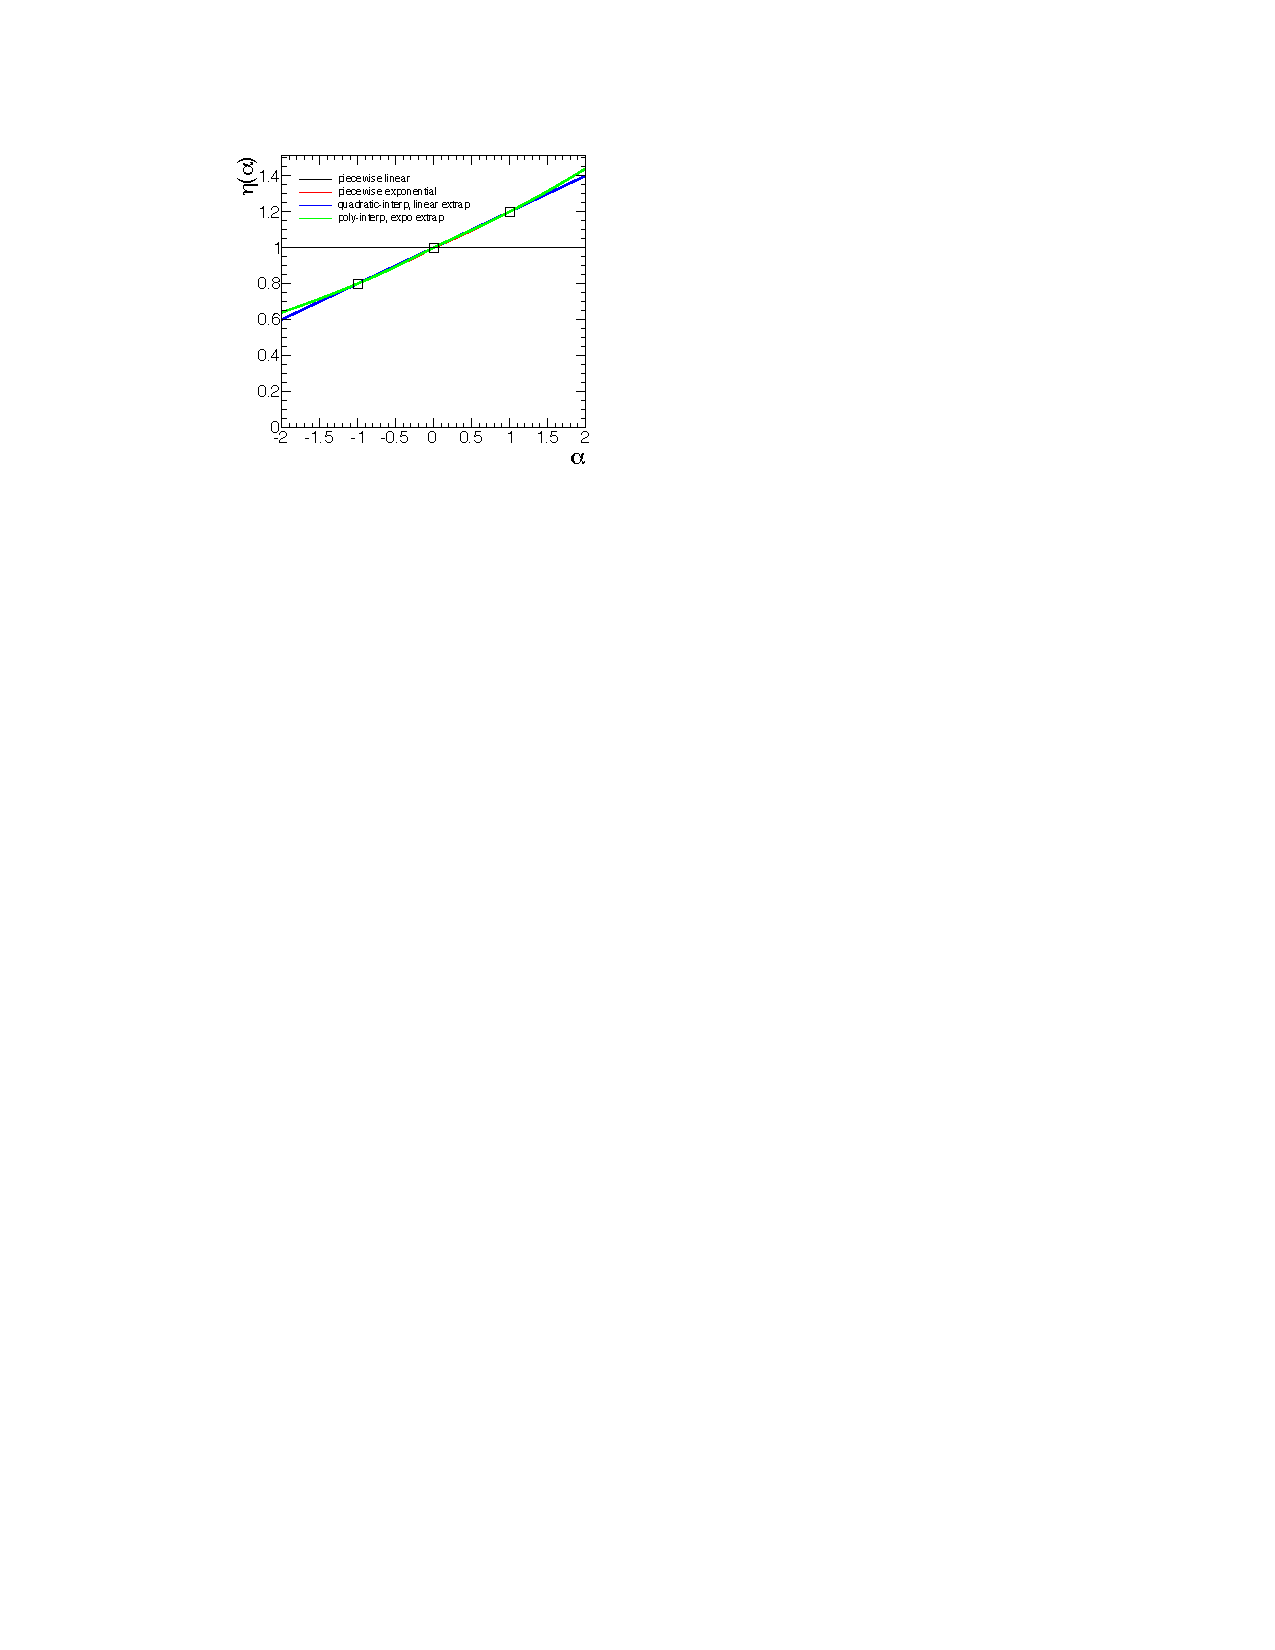
\includegraphics[width=0.4\textwidth]{figures/stat/interp_1.pdf}\label{fig:interp_1}}
\subfigure[]{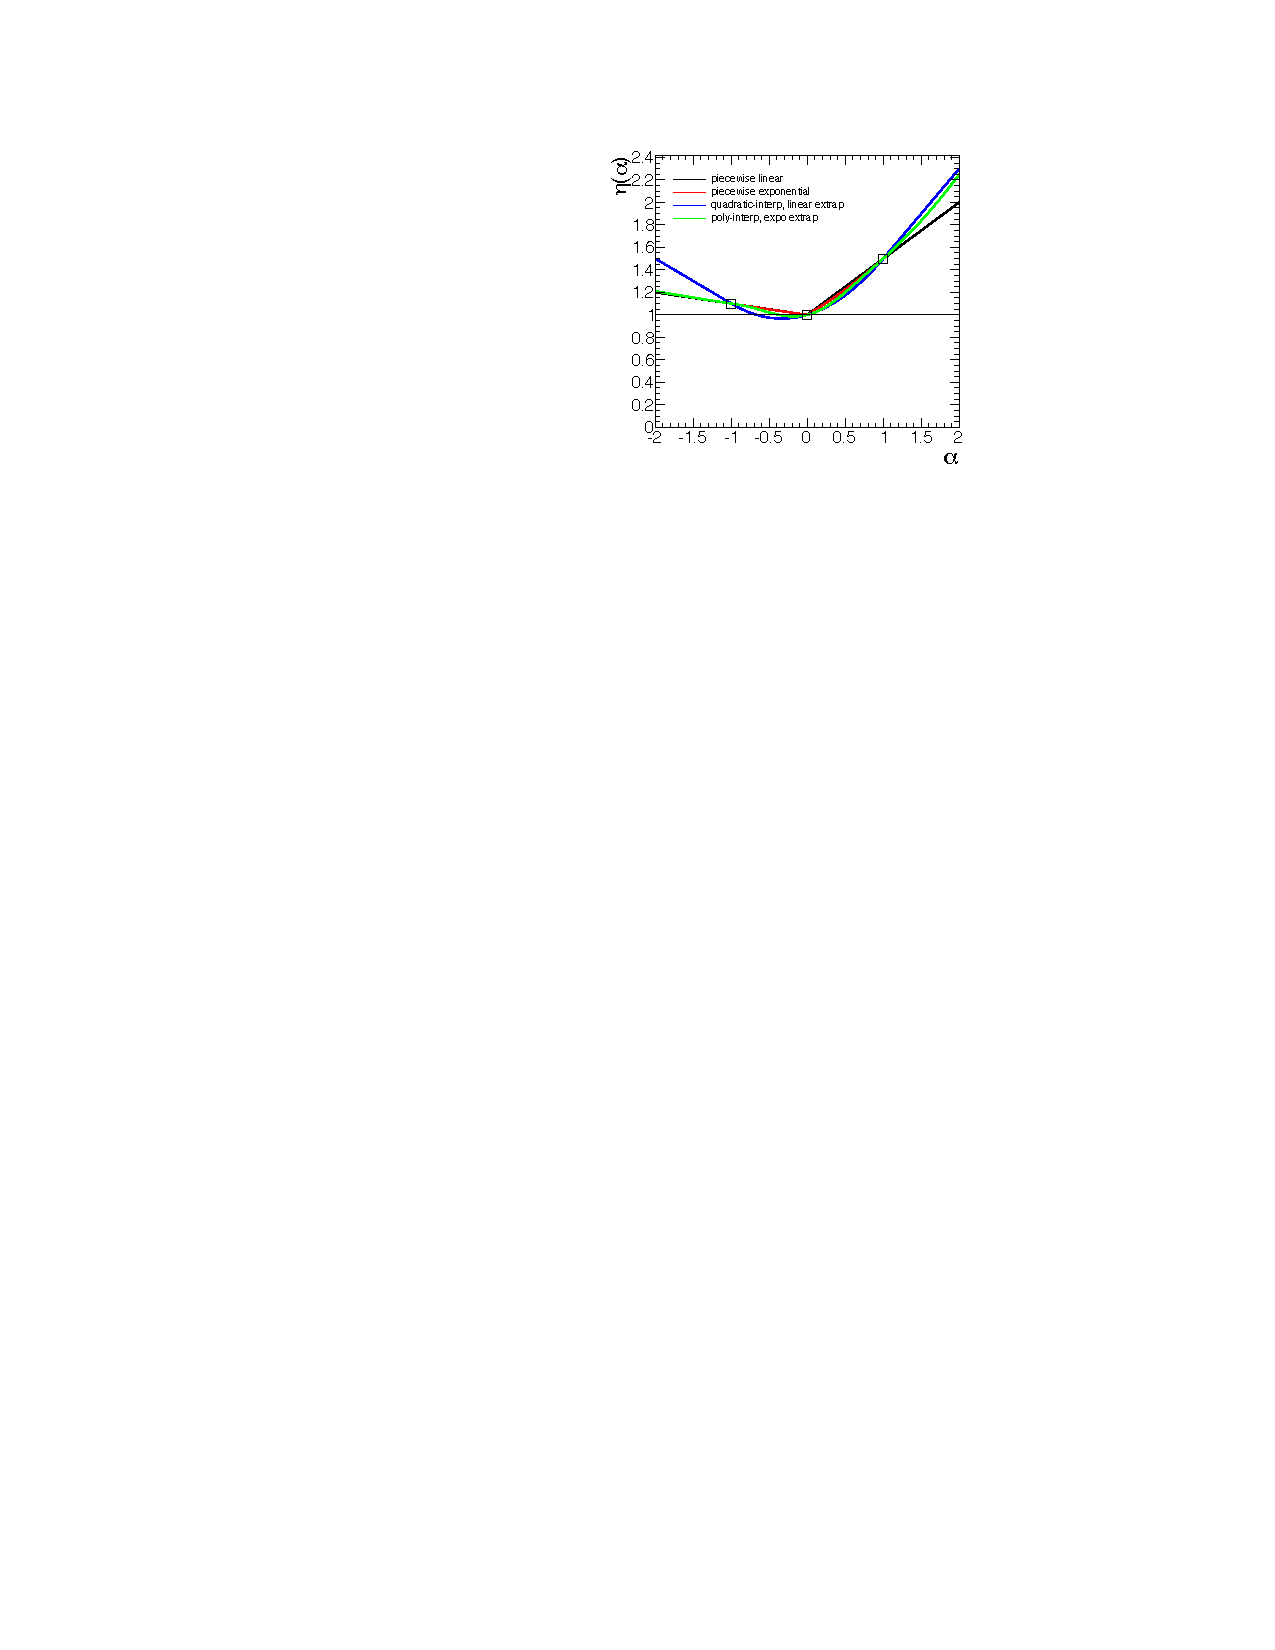
\includegraphics[width=0.4\textwidth]{figures/stat/interp_2.pdf}\label{fig:interp_2}}
\subfigure[]{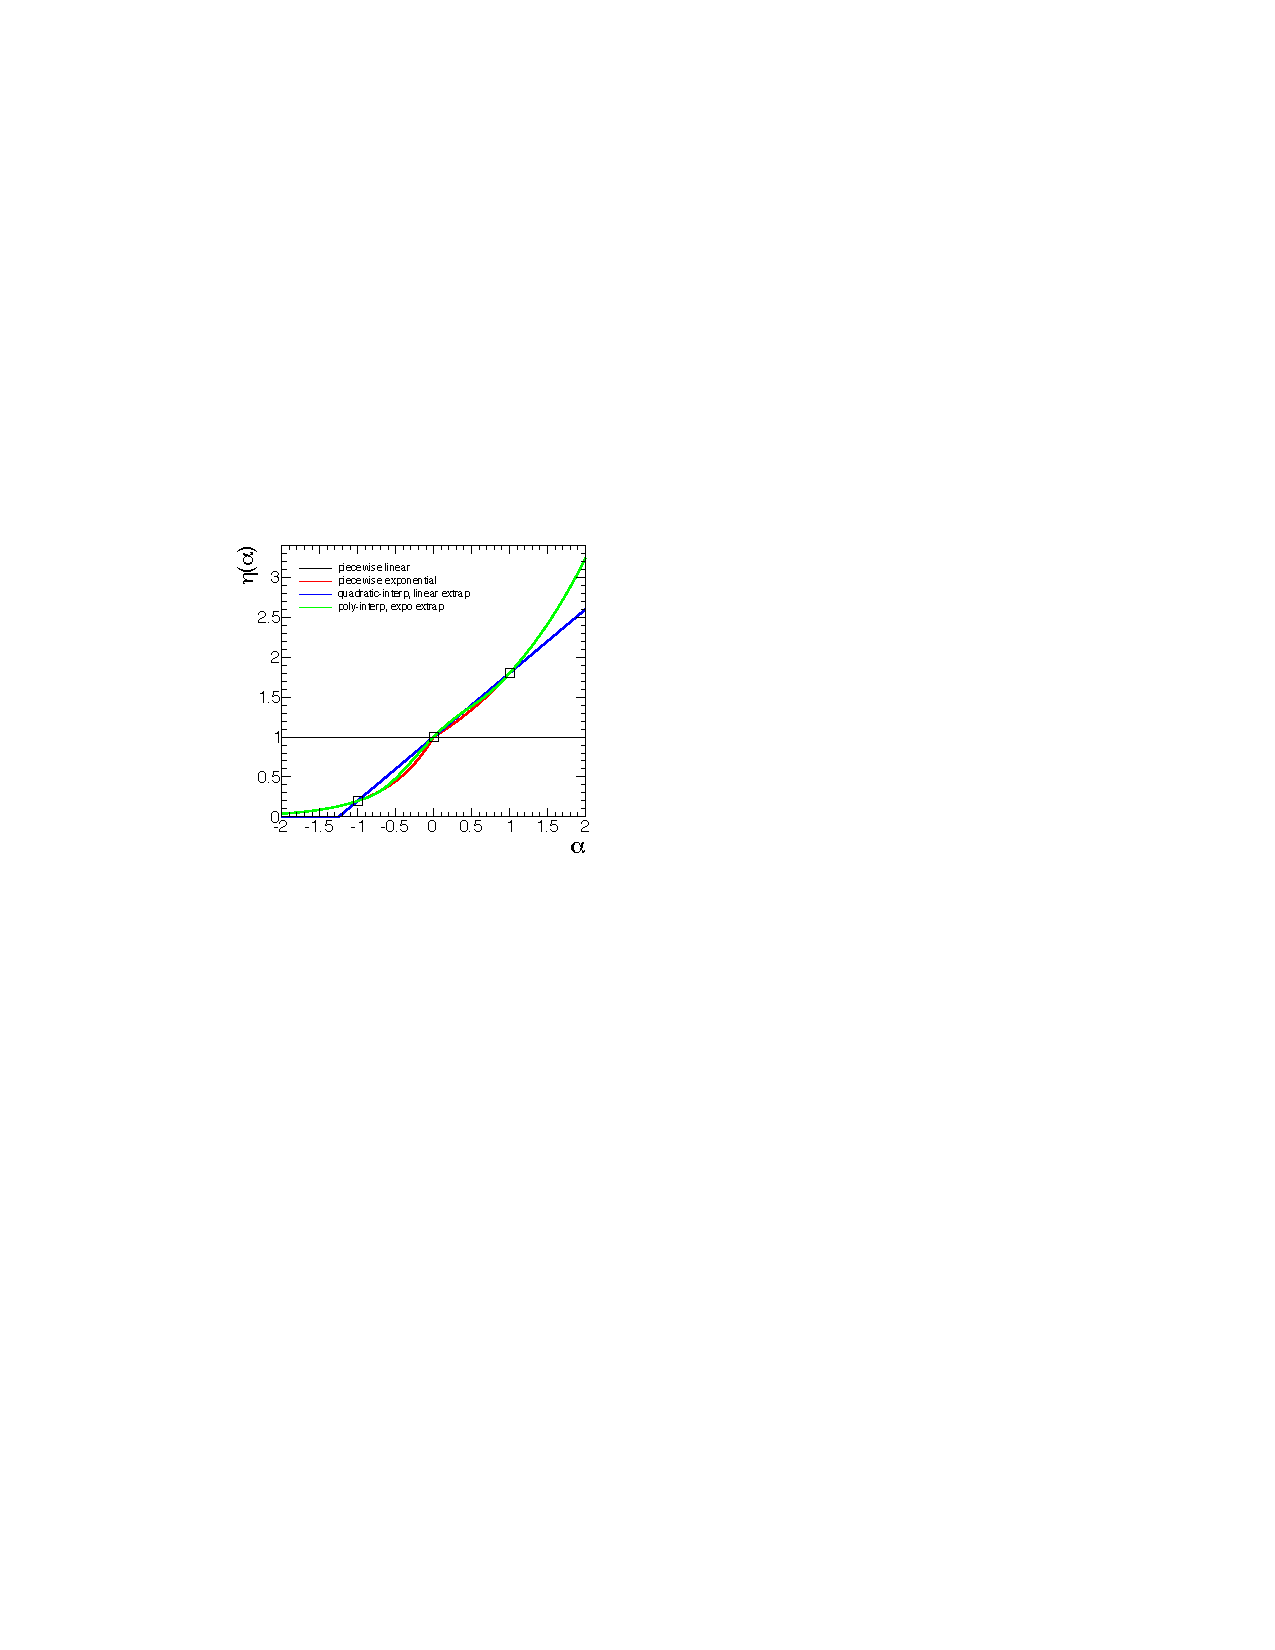
\includegraphics[width=0.4\textwidth]{figures/stat/interp_3.pdf}\label{fig:interp_3}}
\subfigure[]{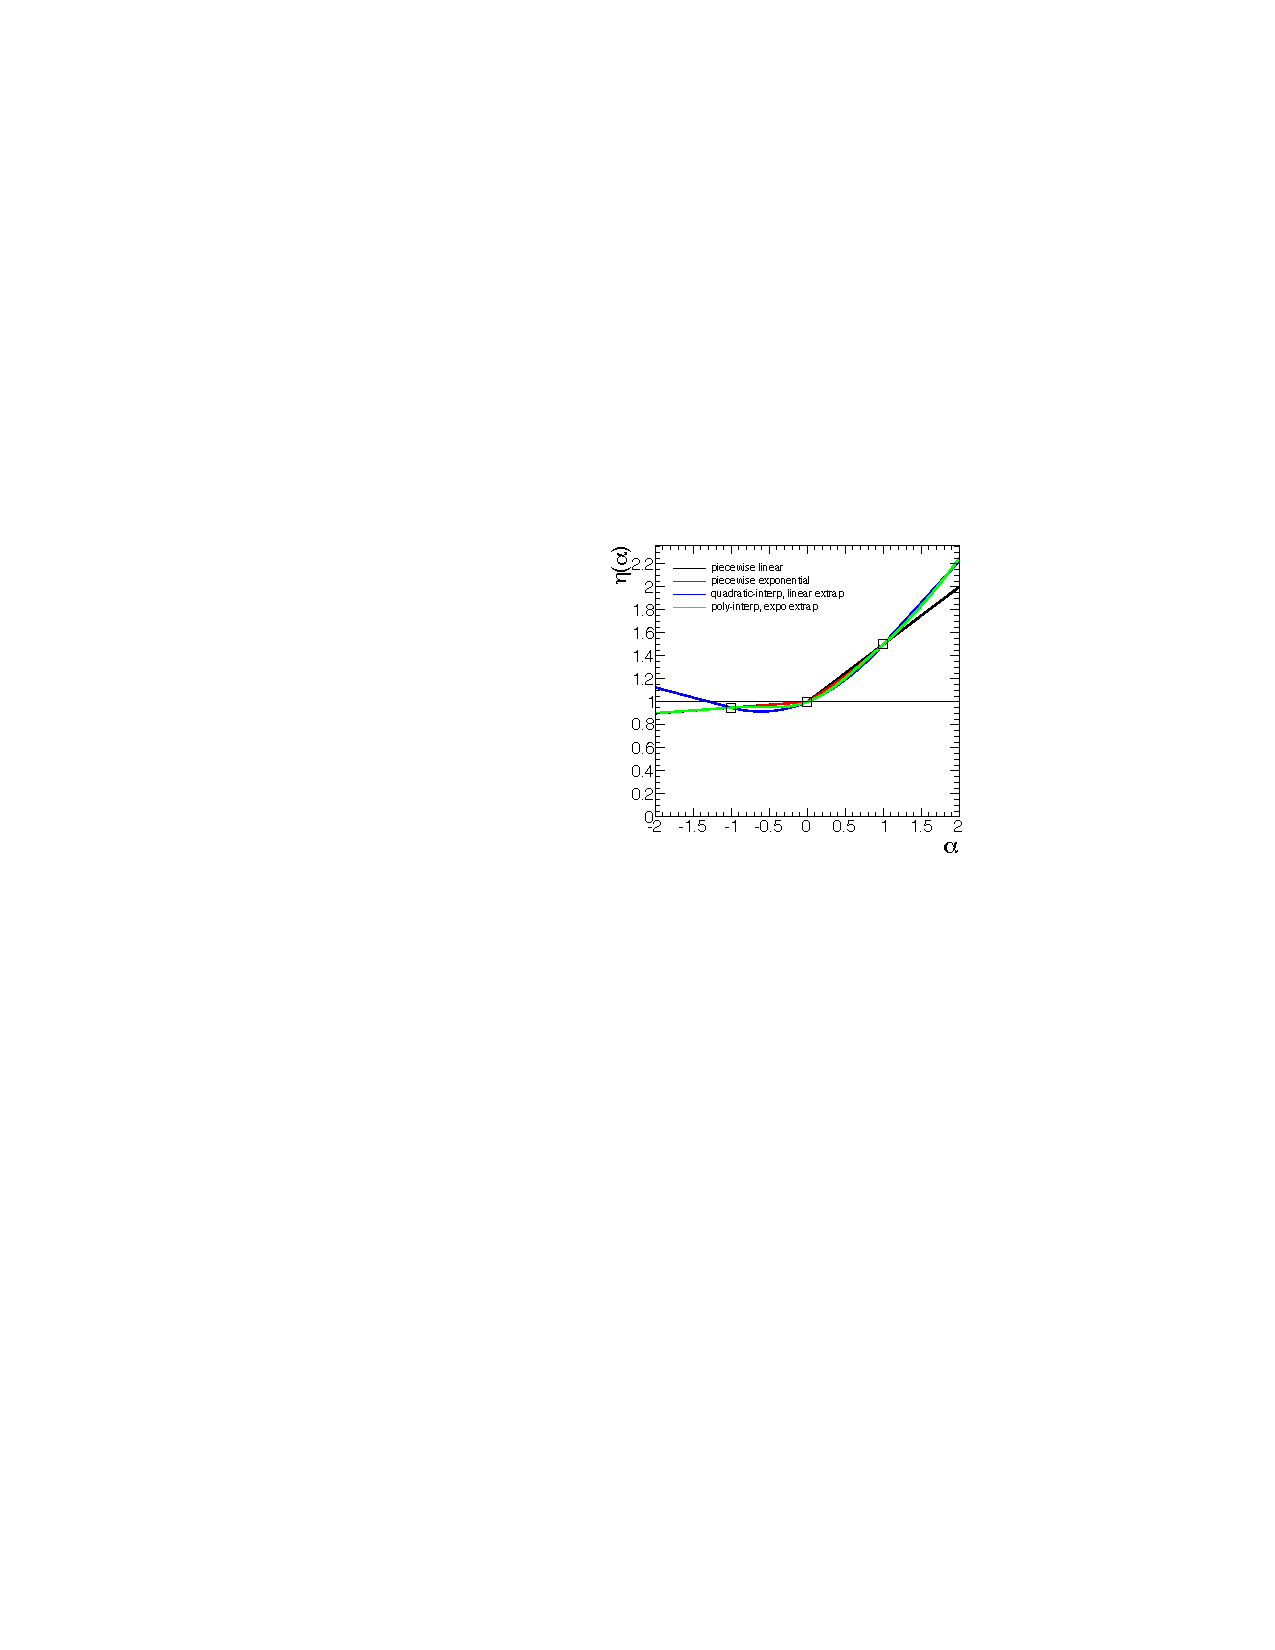
\includegraphics[width=0.4\textwidth]{figures/stat/interp_4.pdf}\label{fig:interp_4}}
\caption{Comparison of the four interpolation options described in the text. $\alpha$ represents the variation of the \gls{np} in units of standard deviations, and $\eta$ the response relative to the nominal value; the three white markers are the points where the response is measured (nominal and $\pm$ one sigma), while the colored lines show the interpolating function.
\subref{fig:interp_1} $\eta(-1) = 0.8$, $\eta(+1) = 1.2$.
\subref{fig:interp_2} $\eta(-1) = 1.1$, $\eta(+1) = 1.5$.
\subref{fig:interp_3} $\eta(-1) = 0.2$, $\eta(+1) = 1.8$.
\subref{fig:interp_4} $\eta(-1) = 0.95$, $\eta(+1) = 1.5$.
Figures from Ref. \cite{Cranmer:1456844}.
}
\label{fig:stat:interp}
\end{figure}


\subsubsection*{Correlation and profiling}

The post-fit values of the \glspl{np} can be compared to the pre-fit values. A central value close to 0 and an uncertainty close to 1 indicates that the fit does not have enough statistical power to profile the uncertainties. If the central values is different from 0, it means that the best value is different from the nominal one; the modified \gls{mc} will have a better agreement with data than the original one. If the post-fit uncertainty on one \gls{np} is smaller than 1, it means that the original assigned uncertainty was too large and the fit was able to constrain the uncertainty on that \gls{np}.
% The effect of a specific systematic is not compatible with the range allowed by the data statistics 

When multiple \glspl{np} have a similar effect on the background prediction, the total variation obtained as a sum of their effects can be larger than what allowed by data. The individual effects can not be disentangled and constrained individually, but a correlation between them produce a total variation that is compatible with what observed in data. % chiarareco:;\ un po' copiato da Javier, rifrasare!


\subsection{Profiled Likelihood Ratio}

Once we divide the parameters in the likelihood into \glspl{poi} and \glspl{np}, the likelihood itself can be maximized globally with respect to both the \gls{poi} and the \glspl{np} ($L(\hat{\mu}, \hat{\theta})$), but we can also find the conditional maximum for a certain value of the \gls{poi} ($L(\mu, \hat{\hat{\theta}})$). The ratio of these two quantities is the \gls{prl}:

\begin{equation}
\label{eq:stat:prl}
\prl = \frac{ L(\mu, \hat{\hat{\theta}}) } {L(\hat{\mu}, \hat{\theta}) } \;.
\end{equation}

\noindent As it was discussed in section \ref{sec:stat:MLE}, rather than maximizing the \gls{prl} it is more convenient to minimize its negative logarithm, $- \loglr$.

%%%%%%%%%%%%%%%%%%%%%%%%%%%%%%%%%%%%%%%

\section{Hypothesis testing}
\label{sec:stat:ht}

Hypothesis testing is the statistical procedure that allows to confirm or reject a specific model. In the case of high-energy physics, a typical example is the identification of the type of a particle based on its energy deposits in the detector. Another example, that will be be used as main test case in this section, is the discovery or exclusion a \gls{bsm} theory. When the alternative between two hypotheses is presented, they are typically indicted as null hypothesis and alternative hypothesis. If what we want to do is to proof the discovery of a new \gls{bsm} signal by excluding the SM only hypothesis, the following symbols are used:

\begin{itemize}
\item[H$_0$] The null hypothesis, corresponds to SM only.
\item[H$_1$] The alternative hypothesis, corresponds to the SM with the addition of the \gls{bsm} process under test.
\end{itemize}

\noindent The test hypothesis can be generalized by including the signal strength $\mu$, that acts as a cross-section scaling; $\mu$=1 corresponds to the \gls{bsm} process with its theoretical cross section, while $\mu$=0 is the SM.

\subsection{Test statistics and p-value}

 A test statistic $t$ is single real-value quantity, function of all the collected data. The \gls{pdf} of the test statistic is different if we assume the null hypothesis or the alternative hypothesis to be true.

To quantify the compatibility of the observed data with a specific model, a p-value can be extracted from the distribution of the test statistics according to a certain hypothesis. For each hypothesis under test and given an observation, the p-value corresponds to the probability of having another observation more extreme than the current one:

\begin{equation}
\label{eq:stat:pval}
p_{\mu} = \int_{t_{{\rm obs}}}^{\infty} f(t | \mu ) \,
d t \; ,
\end{equation}

The p-value is therefore a frequentistic statement on the conditional probability of having higher values for $t$ if the measurement is repeated. When the p-value for the test hypothesis is lower than a predefined threshold, the test hypothesis is excluded. In high energy physics the convention is to set this threshold at 0.05. This corresponds to exclusion at 95\% \gls{cl}. Note that excluding an alternate hypothesis does not mean confirming that the null hypothesis is correct, unless the union of the two covers all the possible phase space.

The threshold to exclude the null hypothesis (SM only) and declare a discovery has to be tighter than the one needed to exclude the test hypotheses (\gls{bsm}). The 0.05 threshold would lead to 5\% of the \gls{bsm} searches to declare a discovery even in the absence of any real \gls{bsm} signal. Instead, the convention is to declare evidence for New Physics when the p-value for the B-only hypothesis is lower than $1.3 \times 10^{-3}$, and discovery when it is lower than $2.9 \times 10^{-7}$.

The significance $Z$ of the p-value can be evaluated by transforming it in the equivalent number of standard deviations of a standard Gaussian needed to have an upper-tail integral equal to the p-value:

\begin{equation}
\label{eq:stat:sig}
Z = \Phi^{-1}(1-p) \; ,
\end{equation} 


\noindent where $\Phi$ is the cumulative of the standard Gaussian. Table \ref{tab:stat:thresholds} summarized the conventional values for the exclusion of a signal hypothesis, the declaration of evidence or discovery of New Physics in terms of p-value and significance.

\begin{table}
\center
\begin{tabular}{|c|c|c|}
\hline 
 & p-value  & $Z$ \\ 
\hline 
\hline 
Exclude test hypothesis & 0.05 & 1.64 \\ 
\hline 
Evidence of New Physics & $1.3 \times 10^{-3}$ & 3 \\ 
\hline 
Discovery of New Physics & $2.9 \times 10^{-7}$ & 5 \\ 
\hline 
\end{tabular}
\caption{Conventional p-value and significance thresholds to exclude a test hypothesis, declare evidence or discovery of New Physics.}
\label{tab:stat:thresholds}
\end{table}




\subsection{Test statistics using the PRL}

While a test statistic can be any real-valued function of the data, the Neyman-Pearson lemma \cite{Neyman} ensures that the ones based on a likelihood ratio are the most statistically powerful. This means that, for a given signal efficiency, they provide the decision criterion that minimizes the misidentification probability. The \gls{prl} defined in Eq. \ref{eq:stat:prl} is the most used at the LHC, and it gives origin to this test statistic:

\begin{equation}
\label{eq:stat:tmu}
t_{\mu} = -2 \log \prl \; ,
\end{equation}

\noindent and the corresponding p-value:

\begin{equation}
\label{eq:stat:pmu}
p_{\mu} = \int_{t_{\mu,{\rm obs}}}^{\infty} f(t_{\mu} | \mu ) \,
d t_{\mu} \; .
\end{equation}

\noindent Different variations of this test statistic are used for discovery and exclusion.

\subsubsection*{Test statistic for discovery}

The discovery test statistics $q_{0}$ used to quantify the level of disagreement of data with the B-only hypothesis in case of an excess is defined as:

\begin{equation}
\label{eq:stat:q0}
q_{0} =
\left\{ \! \! \begin{array}{ll}
               - 2 \ln \lambda(0)
               & \quad \hat{\mu} \ge 0 \;, \\*[0.3 cm]
               0 & \quad \hat{\mu} < 0  \;.
              \end{array} \; \right.
\end{equation}
 
\noindent The reason to assign the value 0 to the test statistic when $\hat{\mu} < 0$ is to avoid excluding the B-only hypothesis in case of a deficit. In fact, $\hat{\mu} < 0$ can indeed be symptomatic of a non correct B-only hypothesis (e.g. a systematic error), but it does not indicate the presence of a signal, which is what we want to highlight with this test statistics. Note that, since \gls{prl} assumes values between 0 and 1, \qzero is positive definite. The associated discovery p-value $p_{0}$ is:

\begin{equation}
\label{eq:stat:p0}
p_{0} = \int_{q_{0,{\rm obs}}}^{\infty} f(q_{0} | 0 ) \, d q_{0} \; .
\end{equation}

\subsubsection*{Test statistics for exclusion}

When investigating the exclusion of the test hypothesis, we want a test statistics that does not penalize an excess. The exclusion test statistics \qmu is therefore defined as:

\begin{equation}
\label{eq:stat:qmu}
q_{\mu} =
\left\{ \! \! \begin{array}{ll}
               - 2 \ln \lambda(\mu)  & \hat{\mu} \le \mu  \;, \\*[0.2 cm]
               0 & \hat{\mu} > \mu \;.
              \end{array}
       \right.
\end{equation}

\noindent This test statistic, also known as one-sided \gls{prl}, is the default one used in the analyses described in the next two chapters. \pmu is consequently defined as the integral above the observed value: 

\begin{equation}
\label{eq:stat:pmu}
p_{\mu} = \int_{q_{\mu,{\rm obs}}}^{\infty} f(q_{\mu} | \mu ) \, d q_{\mu} \;.
\end{equation}

\noindent Note that switching from the discovery test statistic to the exclusion test statistic is equivalent to inverting the role of the background-only and signal-plus-background hypothesis: in the case of the exclusion fit, the null hypothesis to exclude is the signal-plus-background one.

% chiara: e' vero?
% credo che dipenda dal fatto che la L sia simmetrica rispetto a eccessi o deficit
%\noindent Note that, despite the very similar integration formula in \ref{eq:stat:p0} and \ref{eq:stat:pmu}, $p_{\mu, \mu=0}$ is different from \pzero because of the difference in definition between the exclusion and discovery test statistics.

\subsubsection*{Uncapped test statistics}

The strategy described above leads to a loss of information when the test statistic is set to 0. A solution is obtained by uncapping the test statistic and, instead of assigning a 0 to the situations we do not want to penalize, assign them a negative value. This is achieved with the $r_0$ and $r_\mu$ test statistics. As an example, the definition for $r_\mu$ is:
\begin{equation}
\label{eq:rmu}
r_{\mu} =
\left\{ \! \! \begin{array}{ll}
               - 2 \ln \lambda(\mu)  & \hat{\mu} \le \mu  \;, \\*[0.2 cm]
               + 2 \ln \lambda(\mu)  & \hat{\mu} > \mu  \;.
              \end{array}
       \right.
\end{equation}

 
\subsubsection*{Allow only positive signals}

The alternate \gls{prl}, $\tilde{\lambda}({\mu})$, is designed to take into account the fact that, in most physical cases, only positive $\mu$ have a physical meaning. In this case, when $\hat{\mu} < 0$ , the best physical value is 0, and the alternate \gls{prl} is defined as: 

\begin{equation}
\label{eq:stat:lik:alpexcl}
\tilde{\lambda}({\mu}) =
\left\{ \! \! \begin{array}{ll}
               \frac{ L(\mu,
               \hat{\hat{\vec{\theta}}}(\mu)) }
               {L(\hat{\mu}, \hat{\vec{\theta}}) }
                 & \hat{\mu} \ge 0 , \\*[0.3 cm]
                \frac{ L(\mu,
               \hat{\hat{\vec{\theta}}}(\mu)) }
               {L(0, \hat{\hat{\vec{\theta}}}(0)) }
 & \hat{\mu} < 0 \;.
              \end{array}
       \right.
\end{equation}

\noindent The corresponding test statistics are indicated with $\tilde{q}$ and are defined as in Eq \ref{eq:stat:q0} and Eq \ref{eq:stat:qmu} after substituting $\lambda({\mu}) \rightarrow \tilde{\lambda}({\mu})$.

\iffalse
% this equation in the original paper uses the notation t and not q
\begin{equation}
\label{eq:stat:q:excl}
\qmu = - 2 \ln \tilde{\lambda}(\mu) =
\left\{ \! \! \begin{array}{ll}
               - 2 \ln \frac{L(\mu, \hat{\hat{\vec{\theta}}}(\mu))}
                {L(0, \hat{\hat{\theta}}(0))}
                & \quad \hat{\mu} < 0  \;, \\*[0.2 cm]
               -2 \ln \frac{L(\mu, \hat{\hat{\vec{\theta}}}(\mu))}
                {L(\hat{\mu}, \hat{\vec{\theta}})}
&  \quad \hat{\mu} \ge 0  \;.
              \end{array}
       \right.
\end{equation}
\fi

\subsection{The CLs method}

If we consider a situation where $H_0$ and $H_1$ give similar distribution of the exclusion test statistic (e.g. because the signal cross section is
small) and we observe a downward fluctuation in data, we could end up excluding the test hypothesis, even if almost indistinguishable from the null hypothesis. The \gls{cls} method \cite{JUNK1999435} recovers from this situations by defining:

\begin{equation}
\label{eq:stat:cls}
\cls = \dfrac{\pmu}{1 - p_b} , 
\end{equation}

\noindent where $p_b = 1 - p_{\mu, \mu=0}$, as shown in Fig. \ref{fig:stat:pmu_pb}. With the \gls{cls} method, the test hypothesis is excluded at 95\% \gls{cl} if $\cls < 0.05$. In the situation described above, where the null and the test hypotheses give similar \qmu distribution, in case of a deficit both the numerator and the denumerator in Eq \ref{eq:stat:cls} will be small, and the test hypothesis will not be excluded. The \gls{cls} method is the default procedure used in this thesis to decide on the exclusion of a signal model. 


\begin{figure}
\centering
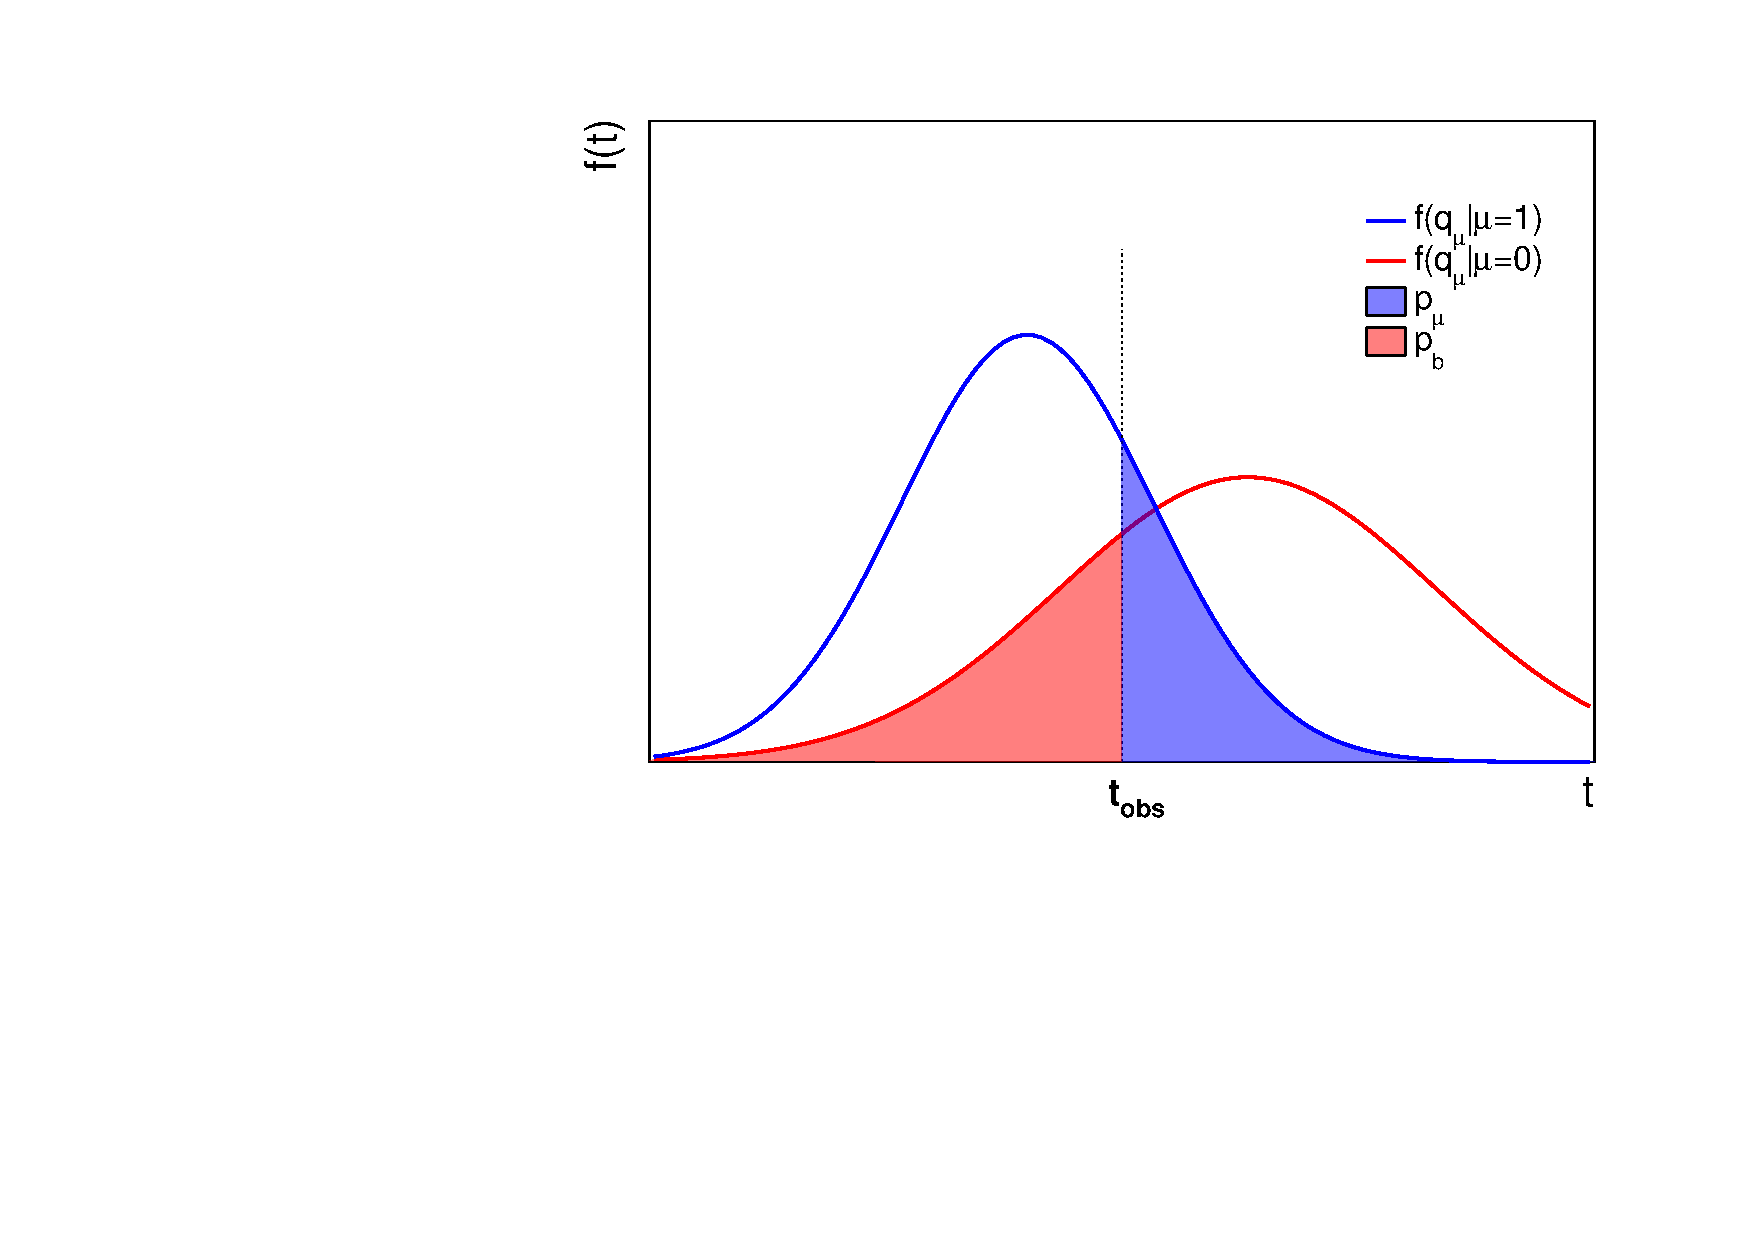
\includegraphics[width=0.7\textwidth]{produce_plots/stat/pmu_pb.pdf}
\caption{Distribution of the test statistic $q_\mu$ in the case of background only (red line) and signal-plus-background (blue line) hypothesis. The filled blue are indicates the value of $p_\mu$, while the filled red area indicated the value of $p_b$.}
\label{fig:stat:pmu_pb}
\end{figure}

\subsection{Distribution of the test statistic}

To compute the p-value associated with the observed value of a test statistics $t$, we need the \gls{pdf} of $t$ assuming that the signal hypothesis $H_\mu$ is true, $ f(t | \mu ) $. The distribution of the test statistics can be obtained with pseudo-experiments or, in the case of large statistics, with the asymptotic approximation. 

\subsubsection*{Pseudo-experiments}

The distribution of the test statistic can be obtained by sampling the likelihood function with \gls{mc} simulations (pseudo-experiments). This is obtained by repeating many times the following steps:
\begin{itemize}
\item The nominal value of all the \glspl{np} is varied by sampling randomly their constraining terms.
\item The new value of the \glspl{np} is used to compute a new expected value for the yields.
\item The observed value is substituted by a Poisson fluctuation of the expected yields.
\item The test statistic for this "observed" value is computed.
\end{itemize}

This is done twice: a first time using as expected number of events the one predicted by the null hypothesis, and a second time the one predicted by the alternate hypothesis. The integral of the two resulting distributions is used to compute the p-values.

\subsubsection*{Asymptotic approximation}
For large number of events, the asymptotic approximation \cite{Cowan2011} can be used to determine the \gls{pdf} of the test statistic without having to simulate several pseudo-experiments. This technique is based on  Wald's theorem \cite{Wald1943}, which states that $t_{\mu} = -2 \ln \lambda(\mu)$ is parabolic up to corrections that scale with the inverse of the square root of the sample size:

\begin{equation}
\label{eq:wald}
t_{\mu} = -2 \ln \lambda(\mu)
= \frac{(\mu - \hat{\mu})^2}{\sigma^2} + {\cal  O}(1/\sqrt{N}) \;.
\end{equation}

\noindent Ignoring the ${\cal  O}(1/\sqrt{N})$ terms, $t_{\mu} = -2 \ln \lambda(\mu)$ is then distributed according to a noncentral chi-square distribution with one degree of freedom:

\begin{equation}
\label{eq:stat:ftmulambda}
f(t_{\mu};\Lambda) = \frac{1}{2 \sqrt{t_{\mu}}} \frac{1}{\sqrt{2 \pi}}
\left[ \exp \left( - \frac{1}{2}
\left( \sqrt{t_{\mu}} + \sqrt{\Lambda} \right)^2 \right) +
\exp \left( - \frac{1}{2} \left( \sqrt{t_{\mu}} - \sqrt{\Lambda} \right)^2
\right) \right] \;,
\end{equation}

\noindent where the noncentrality parameter $\Lambda$ is:

\begin{equation}
\label{eq:stat:noncentrality}
\Lambda = \frac{(\mu - \mu^{\prime})^2}{\sigma^2} \; .
\end{equation}

\noindent The value of $\sigma$ can be estimated through the Asimov dataset, defined as the dataset that, when used to estimate the likelihood parameters, leads to their true values. Plugging this back into Equation \ref{eq:stat:ftmulambda} allows to obtain a functional form of the distribution of the test statistic. Figure \ref{fig:stat:asymtoys1} compares the distribution of the test statistic $q_1$ with pseudo-experiments and with the asymptotic approximation in the case of the background-only hypothesis and in the signal-plus-background hypothesis
in a cut-and-count experiment with nine background events and six signal events; 
it can be observed that a dataset of this size leads to a good agreement of the asymptotic approximation with the \gls{pdf} obtained with pseudo-experiments.
Figure \ref{fig:stat:asymtoys2} shows a further investigation of this comparison: the discovery significance obtained for $q_0=16$ with pseudo-experiments and with the asymptotic approximation is compared as a function of the number of events. 
Even if the approximations used to derive the asymptotic formulae hold in the case of a large data sample, 
the agreement between this method and pseudo-experiments is at the level of $\approx 10\%$ even for an expected background of three events. 


\begin{figure}[h]
\centering 
\subfigure[]{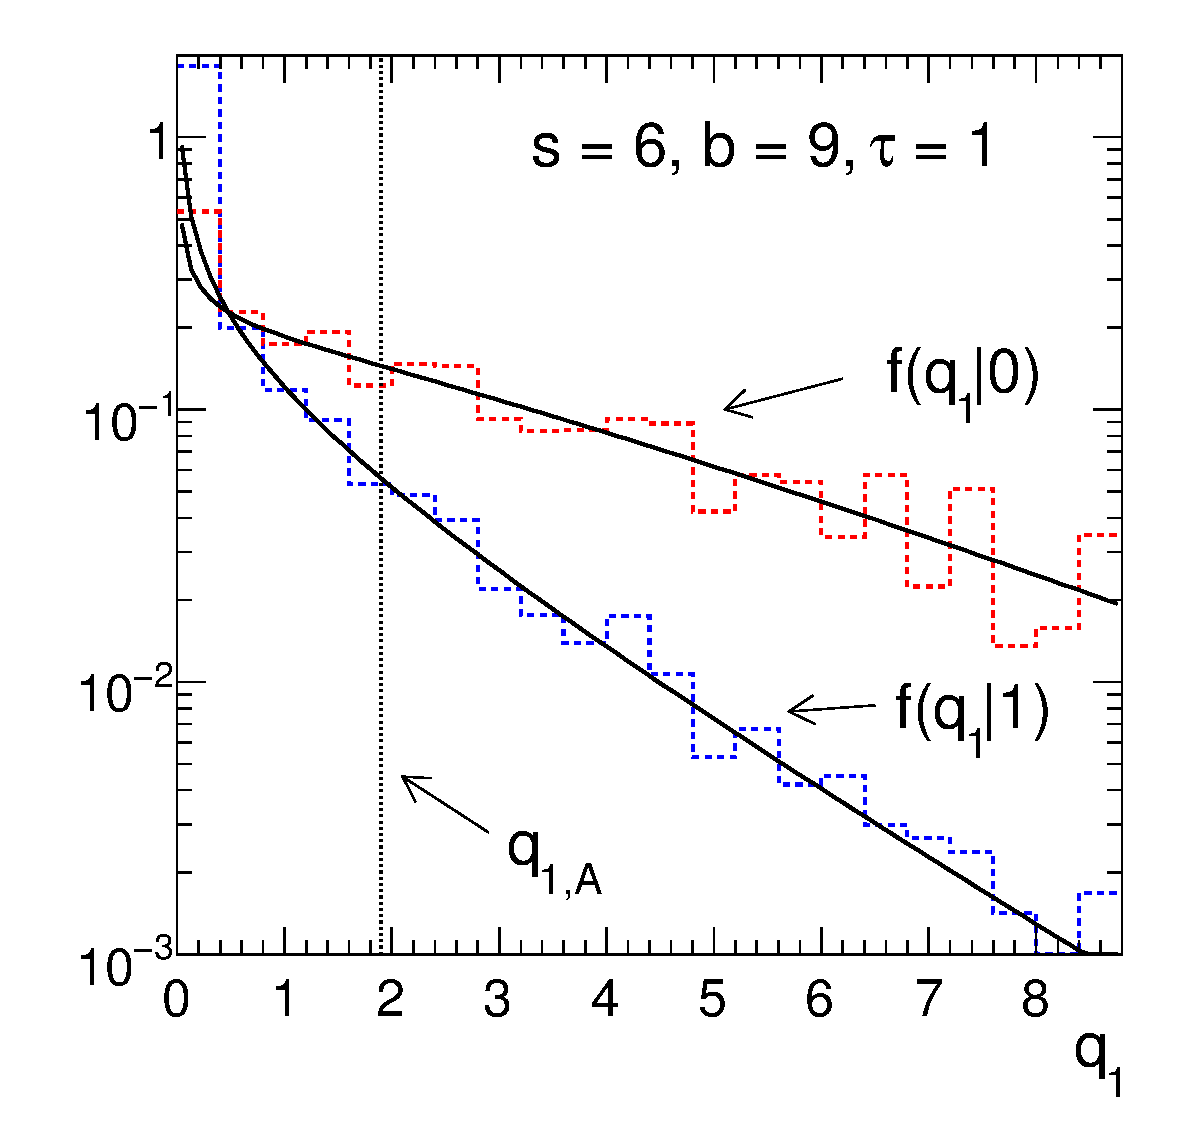
\includegraphics[width=0.48\textwidth]{figures/stat/q11_s6_b9_pdf-eps-converted-to.pdf}\label{fig:stat:asymtoys1}}
\subfigure[]{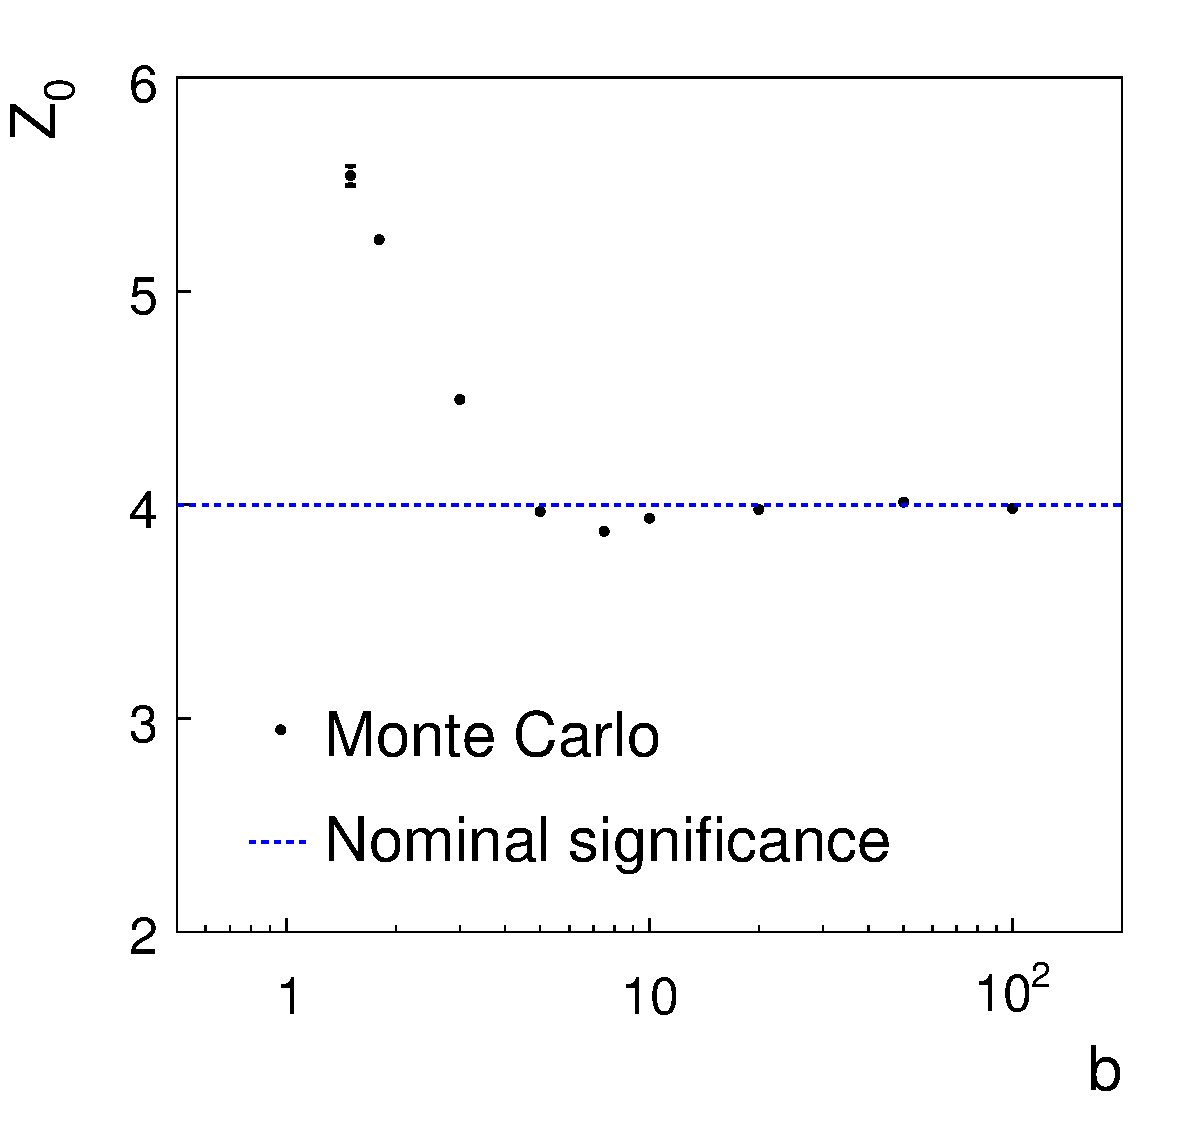
\includegraphics[width=0.48\textwidth]{figures/stat/Z4-eps-converted-to.pdf}\label{fig:stat:asymtoys2}}
\caption{
\subref{fig:stat:asymtoys1} \glspl{pdf} for $q_1$ in the case of the background-only hypothesis and in the signal-plus-background hypothesis
in a cut-and-count experiment with nine background events and six signal events.
The solid curves show the asymptotic approximation, while the histograms are the distributions obtained with pseudo-experiments. 
\subref{fig:stat:asymtoys2} Discovery significance obtained for $q_0=16$ with pseudo-experiments (black points) and with the asymptotic approximation, that leads to a nominal value of $Z_0 = \sqrt{q_0} =4$, as a function of the number of background events. 
Figures from Ref. \cite{Cowan2011}.
}
\label{fig:stat:interp}
\end{figure}



\section{Walk-trough examples}
\label{sec:stat:examples}

In this section we present a few simplified examples that illustrate the concepts described in the previous sections and how they are applied in physics analyses that search for \gls{bsm} signals.
In particular, Section \ref{sec:example_sr} discussed the principle followed in optimizing \glspl{sr}, Section \ref{sec:example_cr} the advantages of using \glspl{cr},
while Section \ref{sec:example_combi} focuses on limit setting and how to improve limits by combining several \glspl{sr}.

\subsection{Region Definition}
\label{sec:example_sr}

\begin{figure}[h]
\centering 
%\subfigure[]{
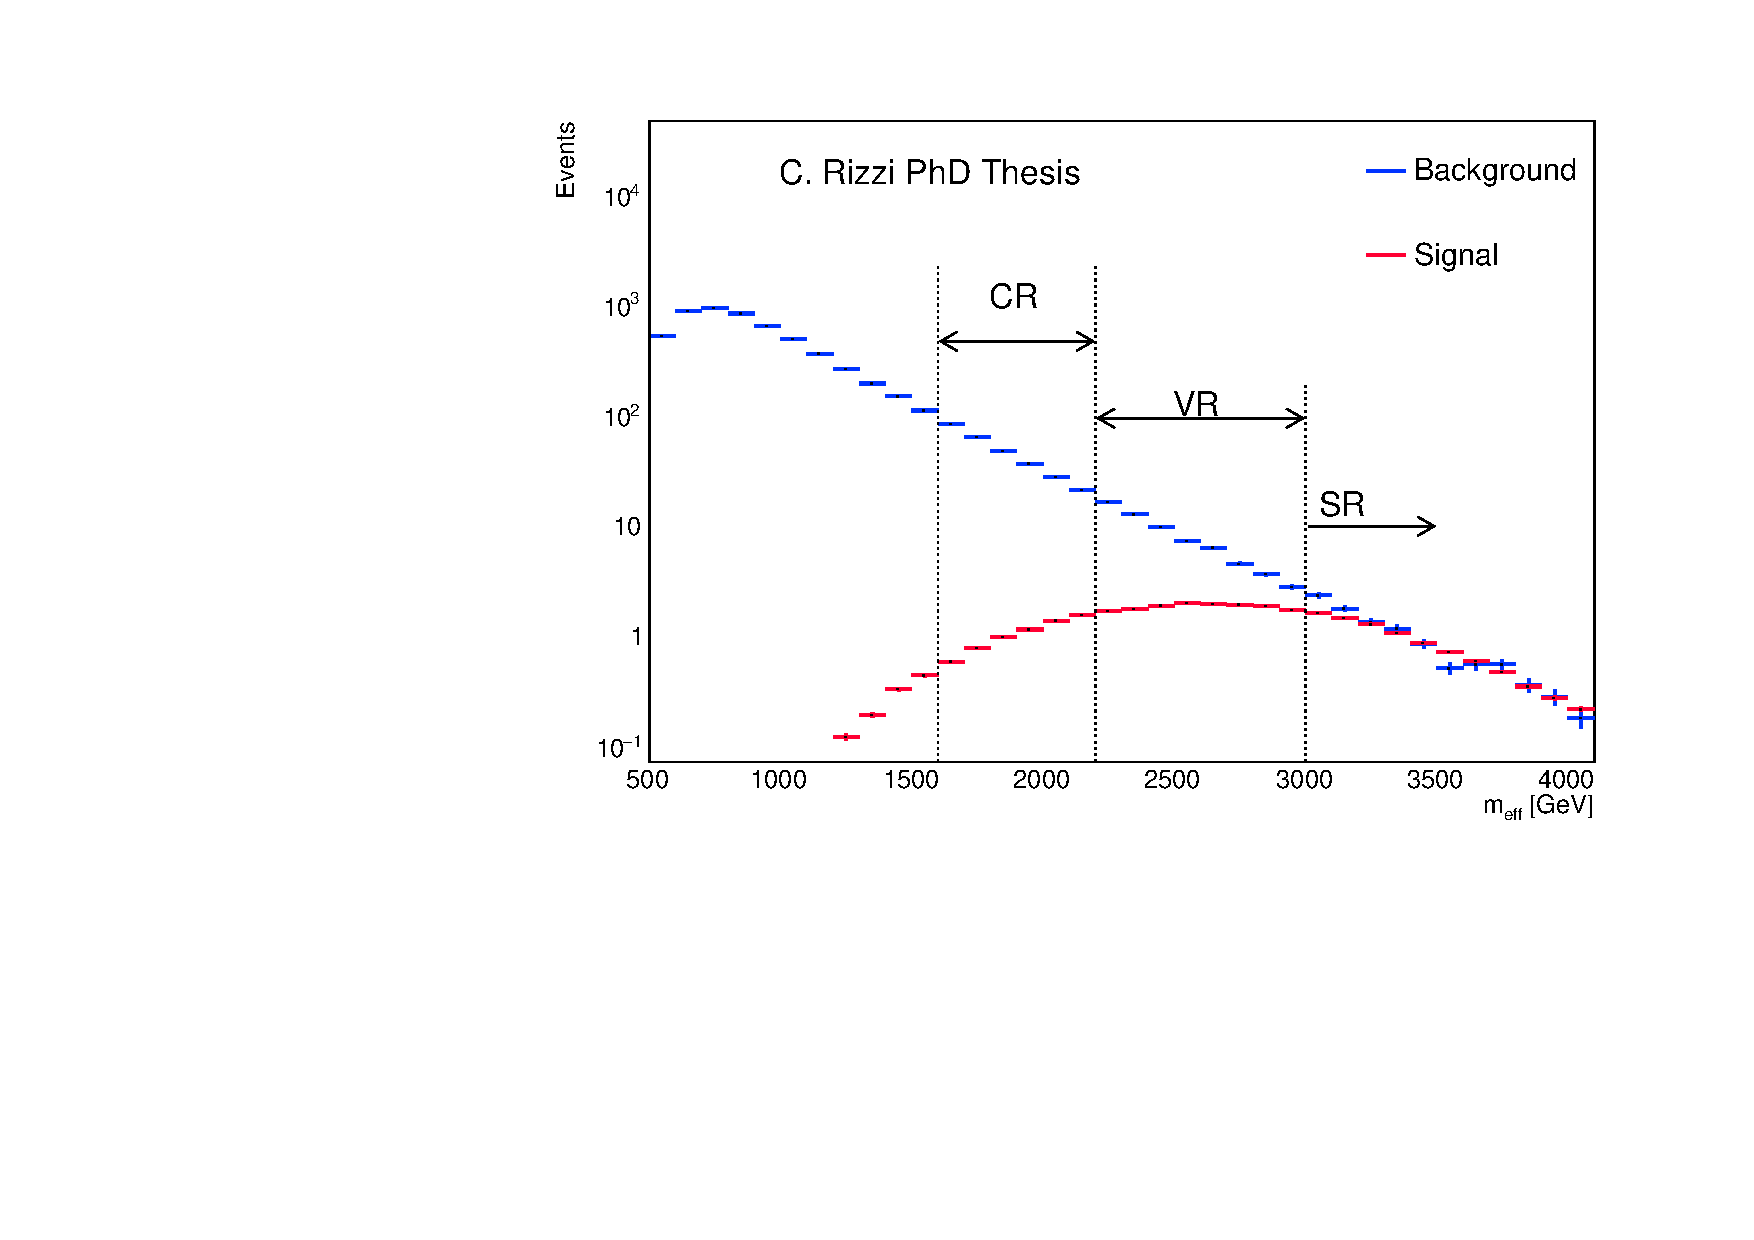
\includegraphics[width=0.6\textwidth]{produce_plots/stat/sig_bkg_CR.pdf}
%\label{fig:stat:example1}}
%\subfigure[]{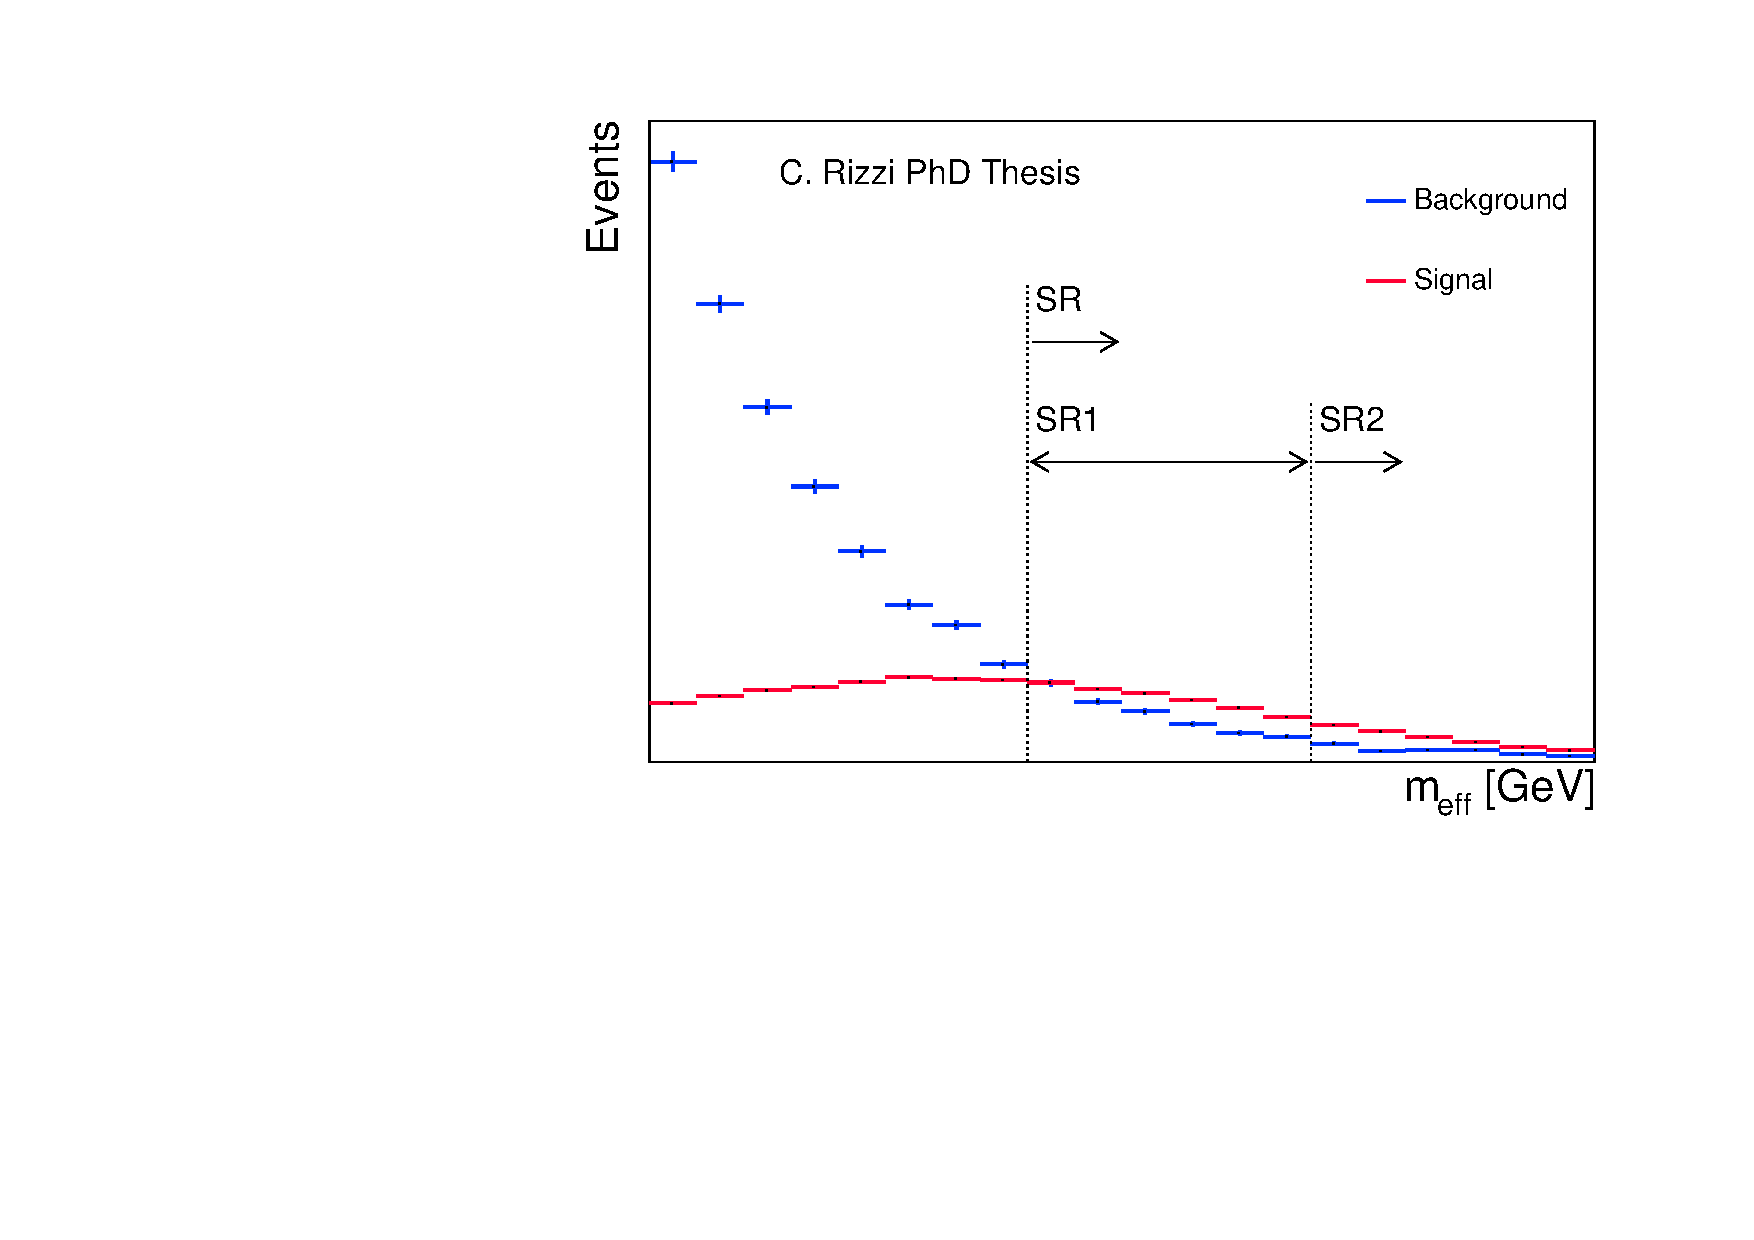
\includegraphics[width=0.48\textwidth]{produce_plots/stat/sig_bkg.pdf}\label{fig:stat:example2}}
\caption{Distribution of a discriminating variable (\meff) for the signal and background in the example in the text. 
The arrows indicate the \gls{sr} defined by maximizing the expected significance and the \gls{cr} where the background is normalized. 
}
\label{fig:stat:example}
\end{figure}

Let's consider a situation where we want to use only one discriminating variable (e.g. \meff) to separate signal and background, 
and they are distributed as in Figure \ref{fig:stat:example}. 
We can see that the background, which in this case we consider as constituted by only one single physical process, 
tends to have lower values of \meff with respect to the signal; 
this means that, to define a \gls{sr}, we will apply a lower selection on the value of \meff.
There are different criteria that can be used to choose the value of \meff that defines the boundary of the \gls{sr}. 
The one used in this thesis is the maximization of the expected significance, computed through the function \binexpZ in \roostats, 
assuming a 30\% uncertainty on the background yields. With this definition, the significance is the equivalent number of standard deviations of a Gaussian of a p-value defined as:

\begin{equation}
\label{eq:binomexpp}
p(N_s, N_b, \sigma_b) = \mathcal{I} \left( \frac{1}{1+ \frac{1}{N_b \sigma_b^2}}; N_s + N_b; \frac{1}{\sigma_b^2} +1  \right)
\end{equation}

\noindent where $N_s$ ($N_b$) is the expected number of signal (background) events, and $\sigma_b$ the relative uncertainty on the background yields and $\mathcal{I}$ the regularized beta function. 

In the case of the signal and background models shown in Figure \ref{fig:stat:example}, values of \meff between 2 TeV and 4 TeV have been tested in steps of 100 GeV, and the optimal value has been found to be $\meff > 3000$ TeV. This selection leads to a \gls{sr} with  9.5 signal events, 10.5 background events and an expected significance of 1.58 $\sigma$. 
The portion of the \meff spectrum that is not occupied by the \gls{sr}, can be used to define a \gls{cr} and a \gls{vr}.
In this example we use the region with $\meff < 2$ TeV as \gls{cr} for the background. 
In order to evaluate the effect of the inclusion of a \gls{cr} in the background estimate, we need to compare the number of expected and observed background event in the \gls{cr}. 
In these examples, the data sample is substituted by a pseudo-data sample generated with a Poisson fluctuation 
of the bin-content of a histogram built as the sum of the background histogram with a scale factor of 0.87 and the signal histogram with a scale factor of 0.5. The summary of the pre-fit background yields, signal yields, signal-to-background ratio, significance and pseudo-data yields in all the regions is given in Table \ref{tab:stat:exampleyeilds}.

\begin{table}
\centering
\begin{tabular}{|c|c|c|c|c|c|}
\hline 
 & CR & VR & SR & SR1 & SR2 \\ 
\hline 
Background & 5775.6 & 83 & 10.5 & 7.4 & 3.1 \\ 
\hline 
Signal & 6.1 & 16.1 & 9.5 & 6.2 & 3.3 \\ 
\hline 
S/B [\%] & 0.1 & 19 & 91 & 84 & 107 \\ 
\hline 
Significance & 0 & 0.38 & 1.58 & 1.32 & 1.20 \\ 
\hline 
Pseudo-data & 4788 & 70 & 15 & 10 & 5 \\ 
\hline 
\end{tabular} 
\caption{Pre-fit background yields, signal yields, signal-to-background ratio, significance and pseudo-data yields in the regions used in the examples in the text.}
\label{tab:stat:exampleyeilds}
\end{table}

\subsection{Background-only fit and control regions}
\label{sec:example_cr}

\glspl{cr} are used first of all in the so called "background-only fit", where the likelihood comprises only the \glspl{cr} and any signal contamination is neglected. The goal of the background-only fit is to extract from the \glspl{cr} data information on the modelling of the background 
and extrapolate it to \glspl{vr} and \glspl{sr}. A background estimate based on a \gls{cr} has two main advantages with respect to the plain \gls{mc} prediction:

\begin{itemize}
\item First of all, the usage of a \gls{cr} allows to eliminate mismodellings in the normalization of the backgorund sample in a phase space 
kinematically close to the \gls{sr}. This is implemented through the inclusion in the likelihood of a normalization \gls{np} with a flat constraint.
The improvement in the description of the data in the \gls{vr} is shown in Figure \ref{fig:stat:VRclosure}: the central value of the bottom panel,
showing the ratio of the pseudo-data to the \gls{mc} simulation, is close to one after the fit.

\item The inclusion of a \gls{cr} in the fit plays a key role also in the evaluation of the systematic uncertainties. 
When computing the impact of a systematic uncertainty in a \gls{sr} or \gls{vr} for a background normalized in a \gls{cr}, 
this does not depend on the full change in yields between the nominal and the systematic variation in that \gls{sr} or \gls{cr},
but it depends only on the change in the \gls{tf}, defined as the ratio of the predicted yields in each \gls{sr}/\gls{vr} to the yields in the \gls{cr}. Figure \ref{fig:stat:VRclosure} shows the reduction of the systematic uncertainty as well: after the fit, the shaded band indicating the uncertainty on the background estimate is smaller.

\end{itemize}

\begin{figure}[h]
\centering 
\subfigure[VR pre-fit]{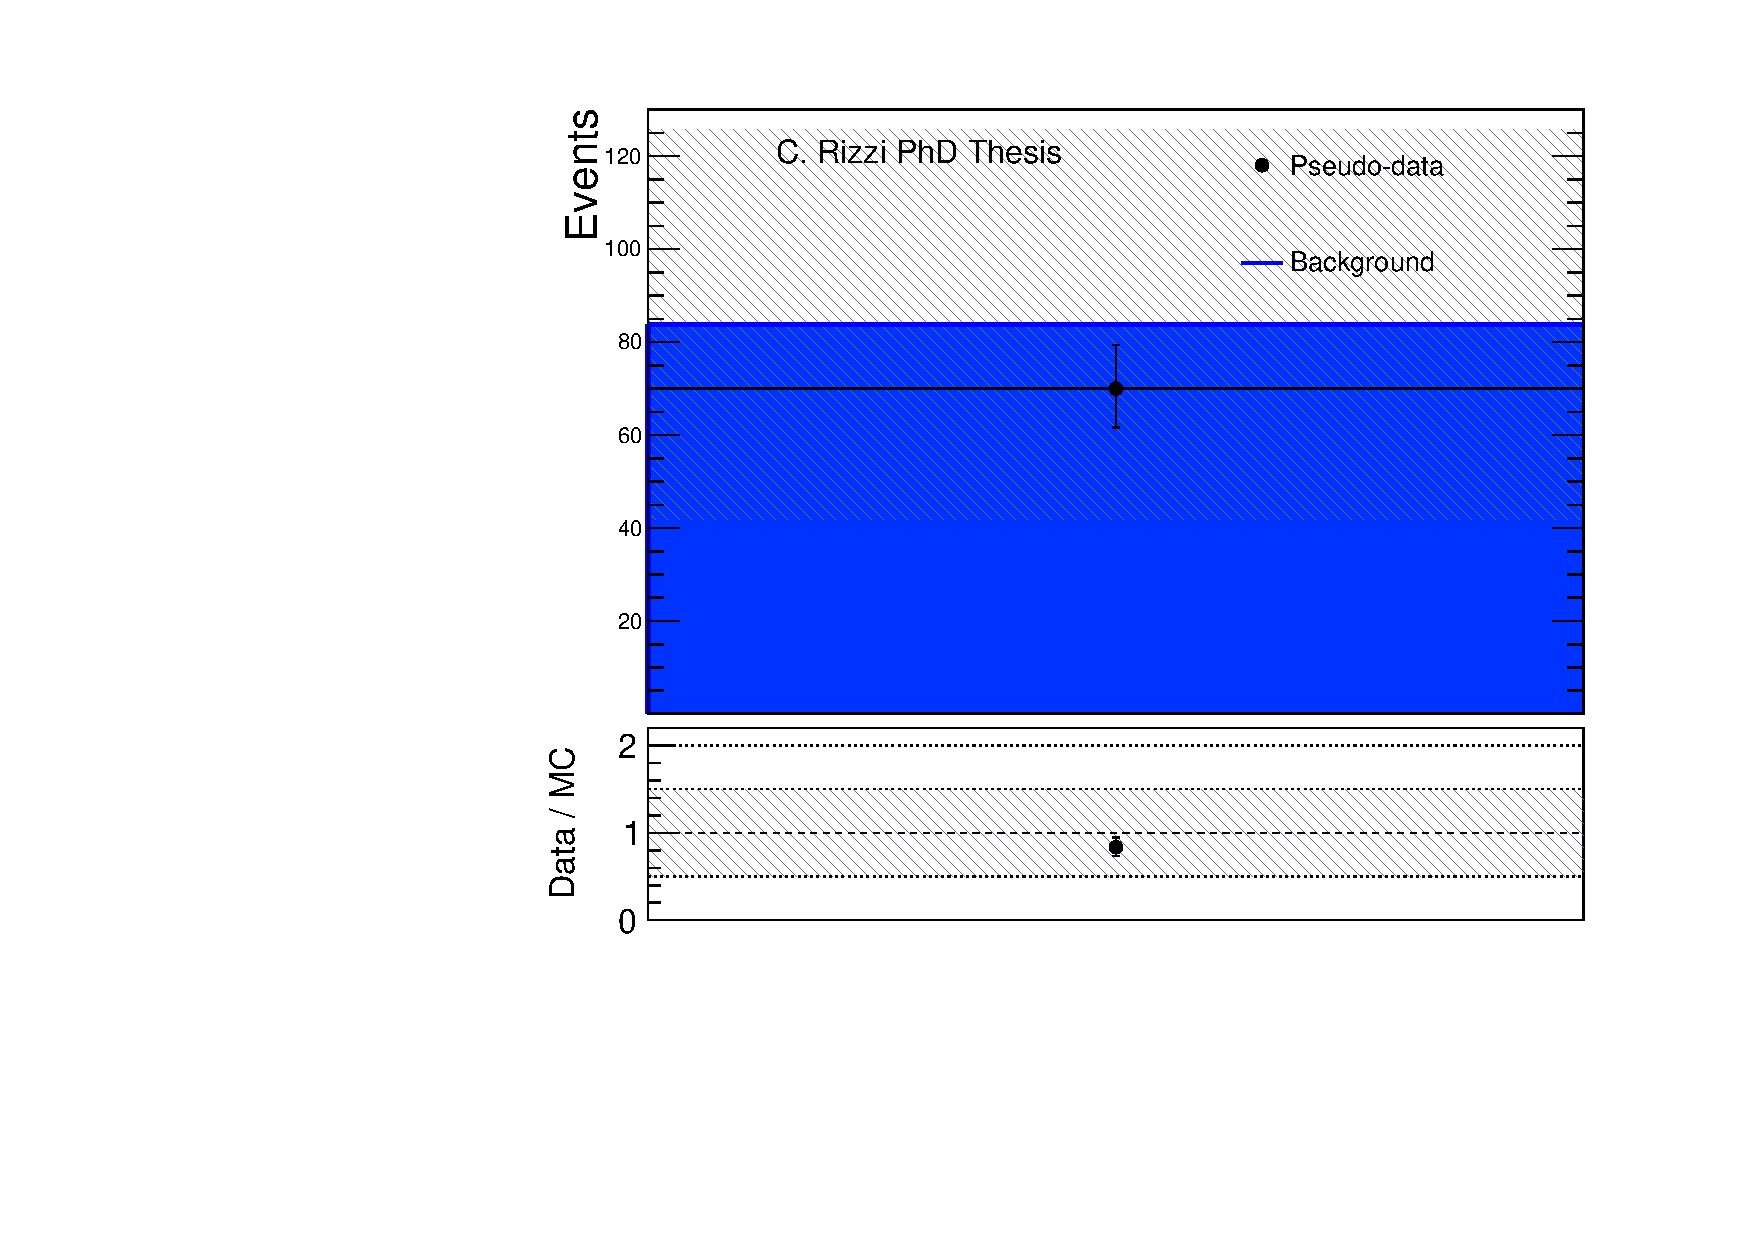
\includegraphics[width=0.4\textwidth]{figures/stat/examples/VR_cuts_beforeFit.pdf}\label{fig:stat:VRprefit}}
\subfigure[VR post-fit]{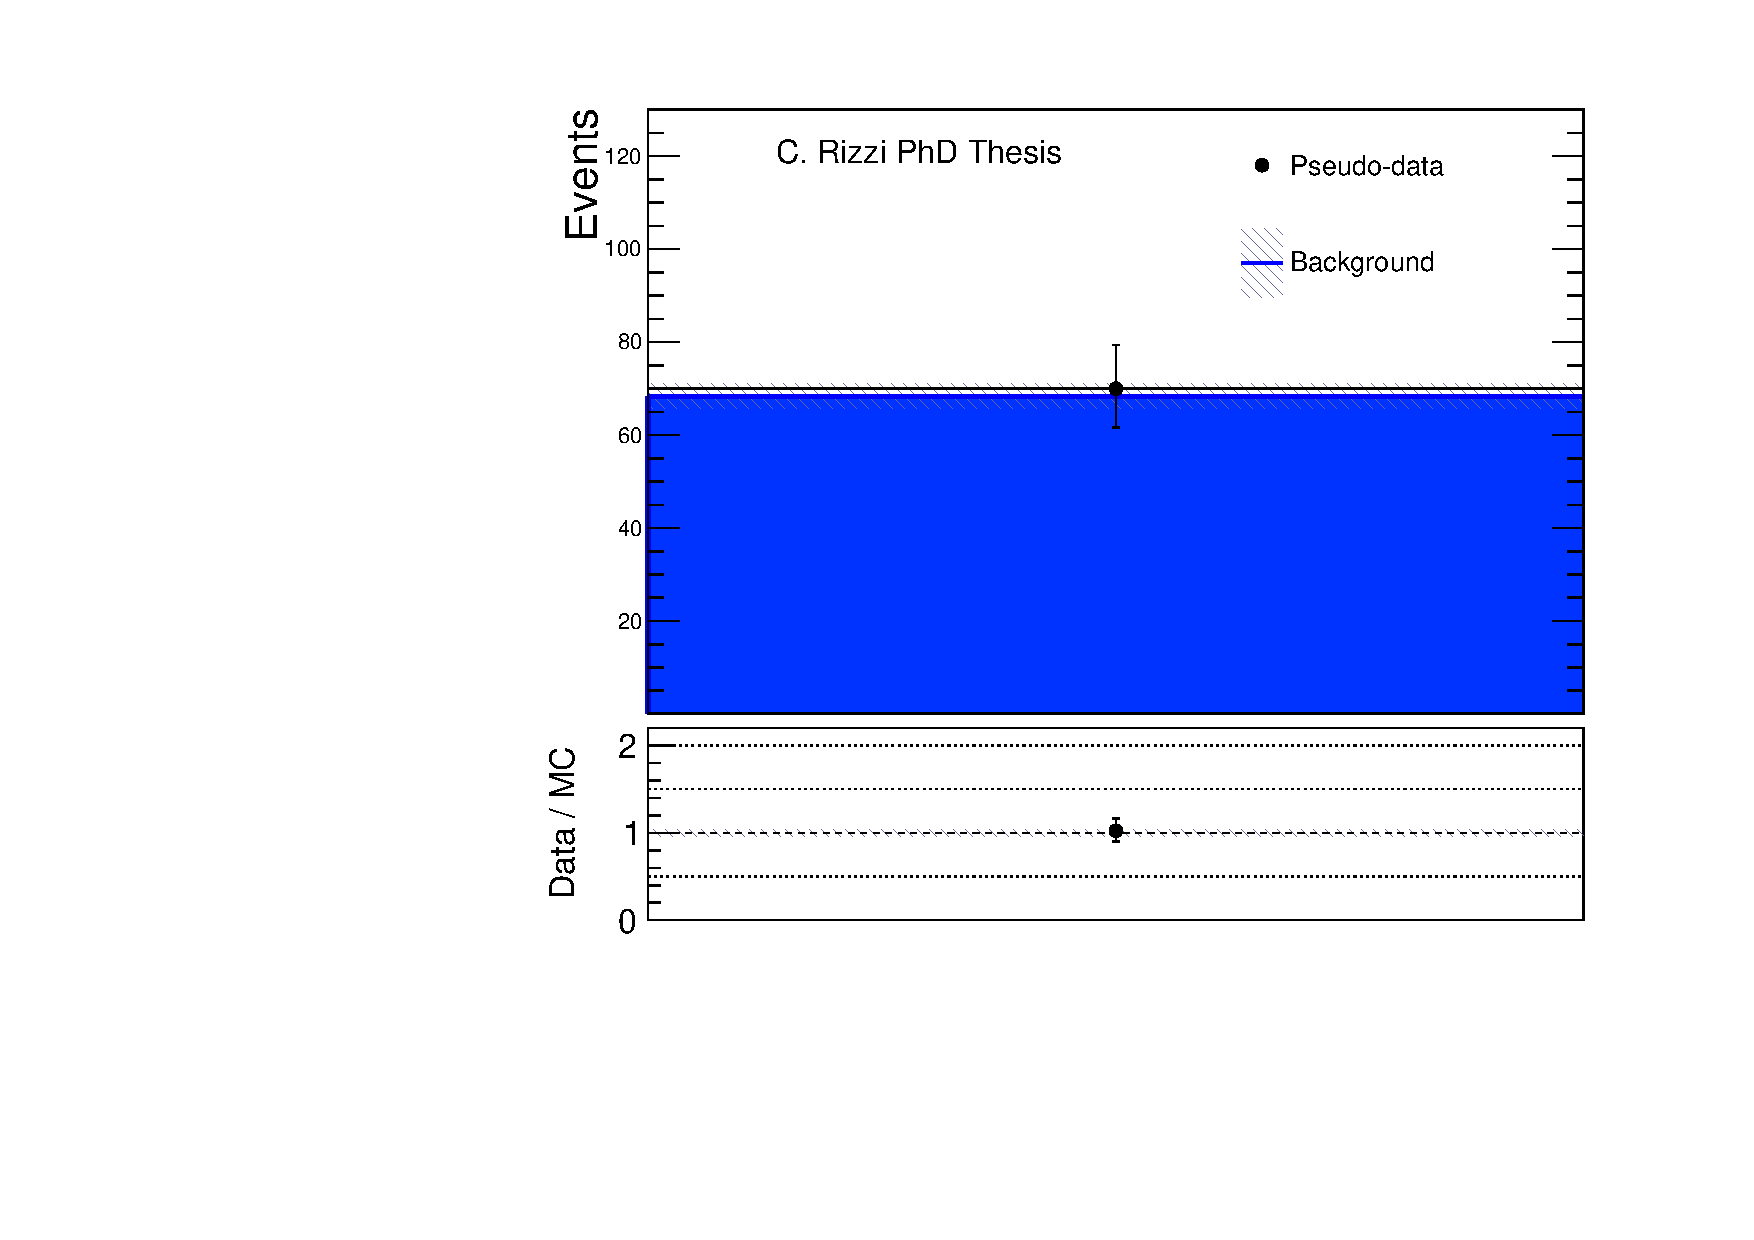
\includegraphics[width=0.4\textwidth]{figures/stat/examples/VR_cuts_afterFit.pdf}\label{fig:stat:VRpostfit}}\caption{
Agreement between \gls{mc} simulation and pseudo-data \subref{fig:stat:VRprefit} before and \subref{fig:stat:VRpostfit} after the fit in the \gls{cr}.
}
\label{fig:stat:VRclosure}
\end{figure}


\subsection{Improving the sensitivity by combining regions}
\label{sec:example_combi}

\begin{figure}[h]
\centering 
%\subfigure[]{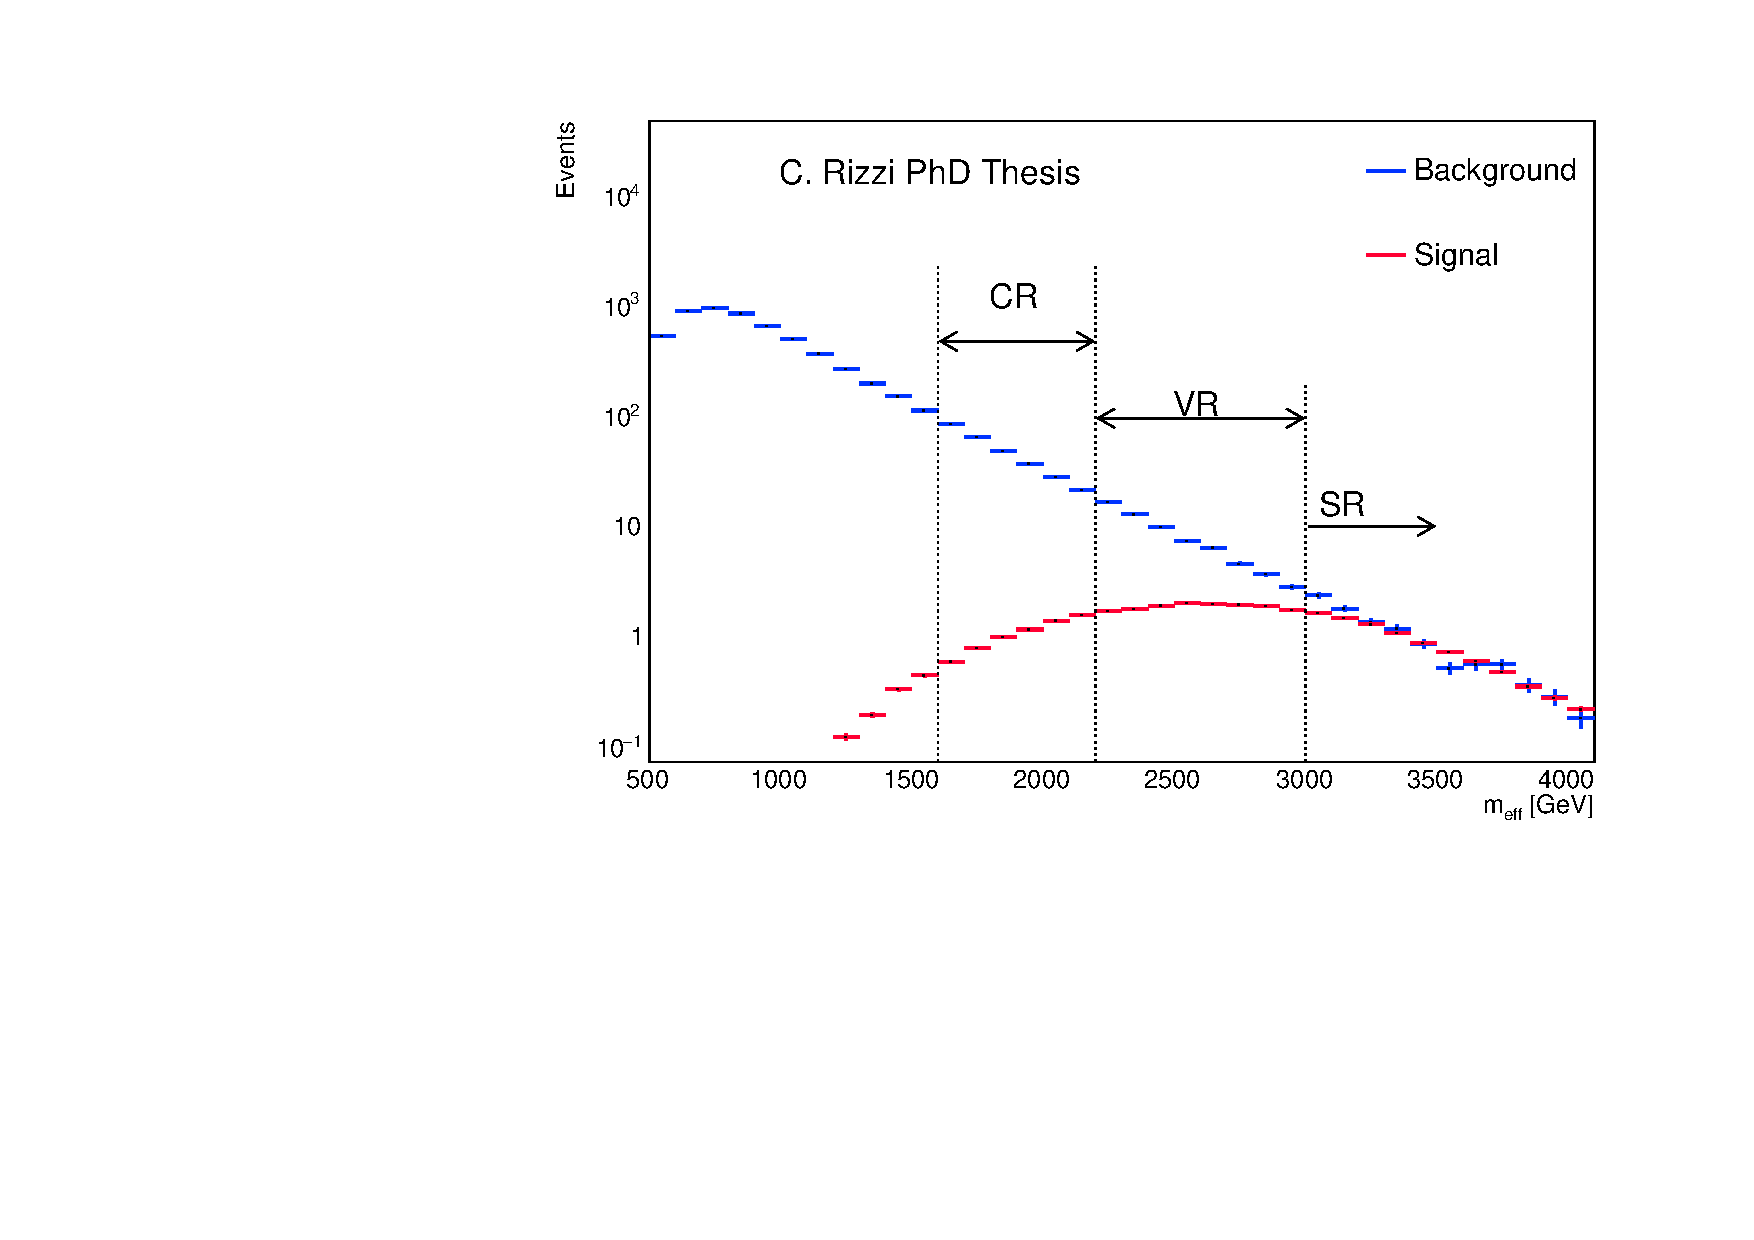
\includegraphics[width=0.48\textwidth]{produce_plots/stat/sig_bkg_CR.pdf}\label{fig:stat:example1}}
%\subfigure[]{
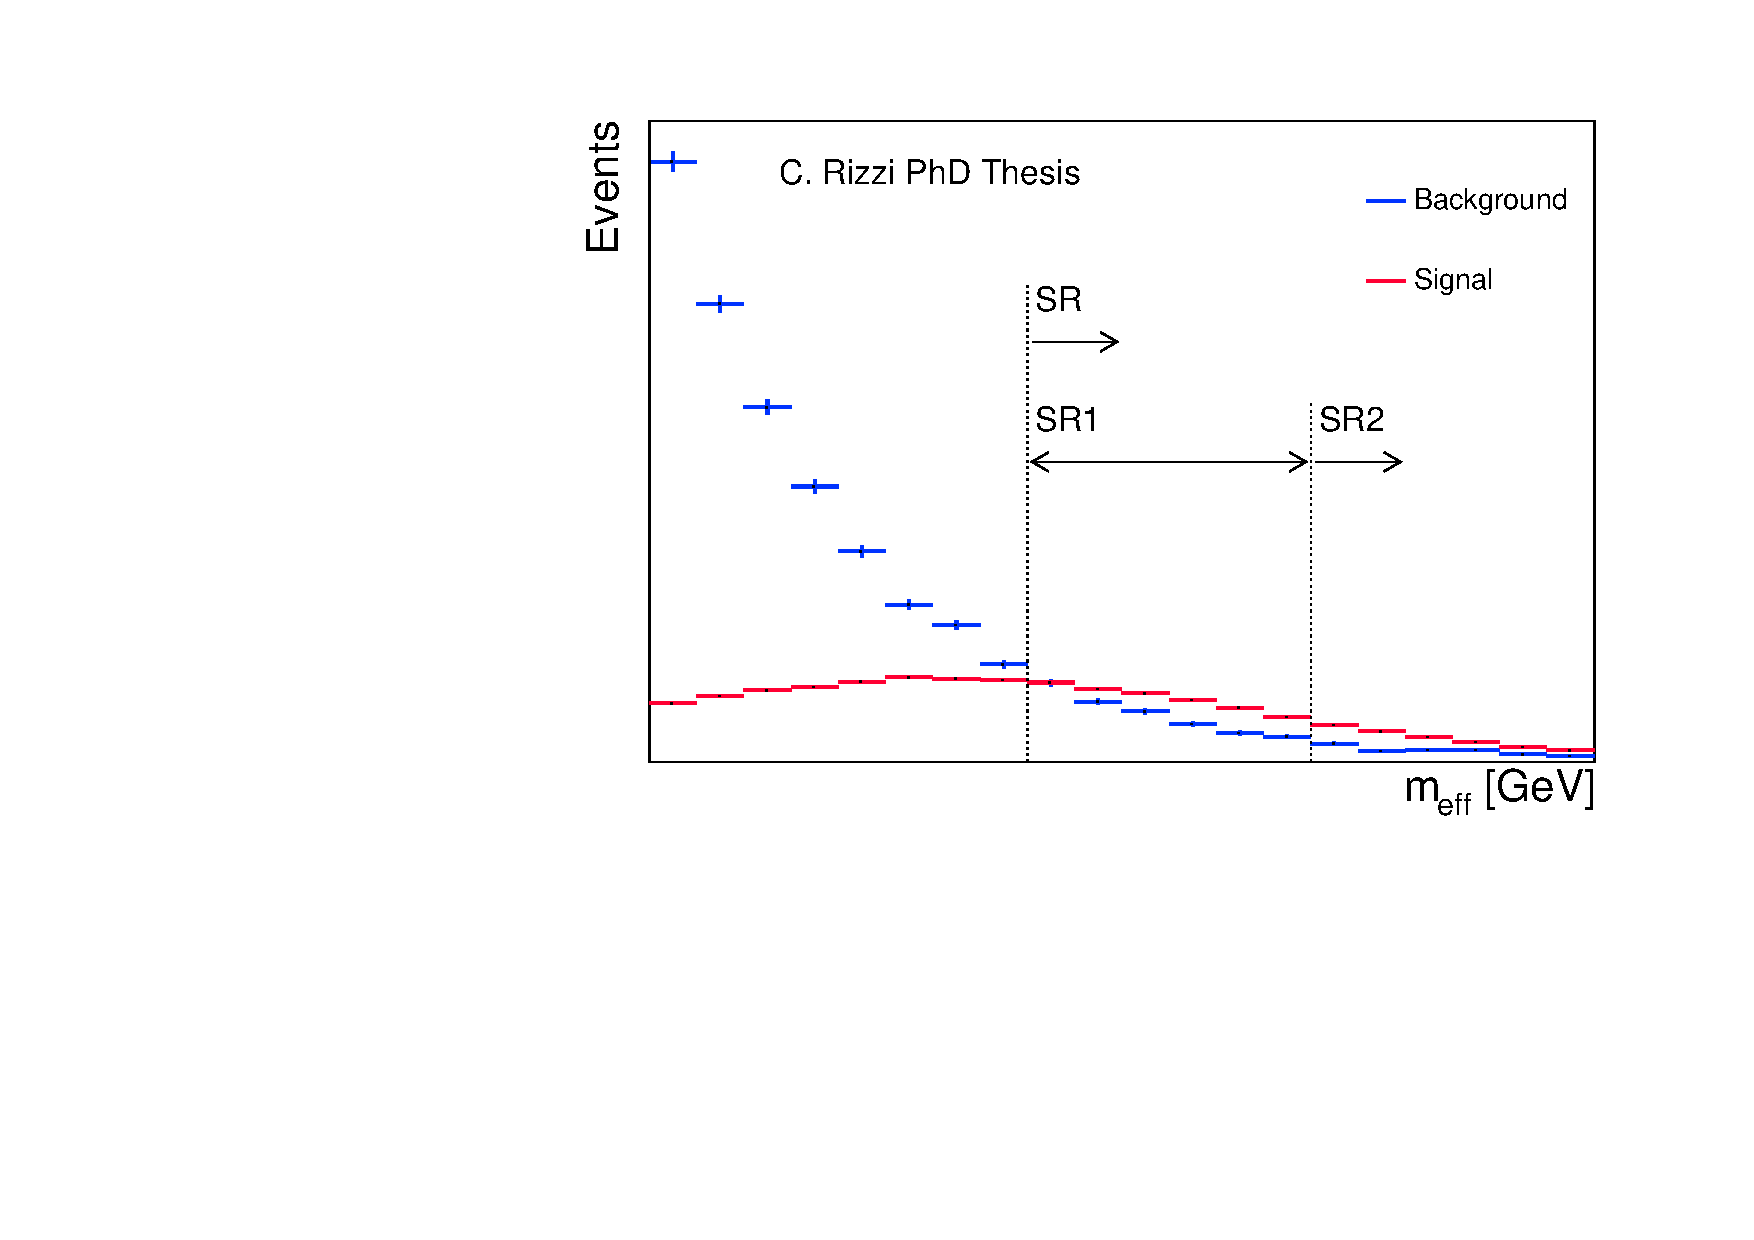
\includegraphics[width=0.6\textwidth]{produce_plots/stat/sig_bkg.pdf}
%\label{fig:stat:example2}}
\caption{
Distribution of a discriminating variable (\meff) for the signal and background in the example in the text.
%\subref{fig:stat:example2} 
The arrows indicate the definition of the \glspl{sr}; the one named "SR" is the region that maximizes the expected significance, while SR1 and SR2 are the orthogonal bins in which SR is divided.
}
\label{fig:stat:example2}
\end{figure}
In this section we show with a simple example how combining different regions can increase the sensitivity. We are going to use the same 




